\vfill\null\columnbreak
\section{Visualisierung}  
    \[u(t)=cos(\omega t) \Rightarrow y(t)=|P(jw)|\cdot cos(\omega t+\angle P(j\omega))\]
  \subsection{Bode Diagramme}
        Die Magnitude und Phase wird gegenüber einer logarithmischen Frequenzskala eingezeichnet.
        Dabei ist die Magnitude üblicherweise in Dezibel, und Die Phase in Grad dargestellt.
        
        \textbf{Umrechnung zwischen dezimal und dezibel:}
        
        \[|\Sigma(s)|_{dB} = 20 \cdot \textrm{log}_{10}|\Sigma(s)|= 20\cdot\frac{\textrm{ln}(|\Sigma(s)|)}{\textrm{ln}(10)}\]
        \[|\Sigma(s)| = 10^{\frac{|\Sigma(s)|_{dB}}{20}}\]
        
        \begin{center}
        {\renewcommand{\arraystretch}{1.4}
            \begin{tabular}{c|c}
        
            Dezimalskala    &   Dezibelskala [dB]\\
            \hline
            100 &   40  \\
            10  &   20  \\
            5   &   13.97..\\
            3.16.. & 10\\
            2   &   6.02..\\
            1   &   0   \\
            $\frac{1}{\sqrt{2}}$  &   -3.0103\\
            0.316.. & -10\\
            0.1 &   -20 \\
            0.01    &   -40\\
            0       &   $-\infty$
            \end{tabular}}
        \end{center}
        \[|\Sigma(j\omega)|_{dB} = |\Sigma_1(j\omega)|_{dB}+|\Sigma_2(j\omega)|_{dB}\]
        \[\angle\Sigma= \angle\Sigma_{1}+ \angle\Sigma_{2}\]
        \[\angle\Sigma(j\omega)=
        \begin{cases}
            \arctan(\frac{x}{y}) & x > 0\\
            \arctan(\frac{x}{y})+\pi & x<0
      \end{cases}
      \]
                 
        \subsubsection{Systeme 1. Ordnung}
            Viele reale Regelkreise können als Systeme erster Ordnung approximiert werden. Ein solches System reagiert auf tiefe Frequenzen, die kleiner als die Eckfrequenz (Cutoff Frequency) $\omega_c = \frac{1}{\tau}$ sind. Bei Anregungsfrequenzen höher als $\omega_c$ verhindert die Trägheit des Systems eine starke Änderung des Ausgangs. Ausserdem reagiert das System für $\omega > \omega_c$ zunehmend verzögert, wie an der Phase des Bode Diagramms ersichtlich ist. Eine wichtiges Merkmal: die Magnitude bei $\omega_c = \frac{1}{\tau}$ ist immer bei $\frac{1}{\sqrt{2}}\approx -3 dB.$
            \begin{center}
                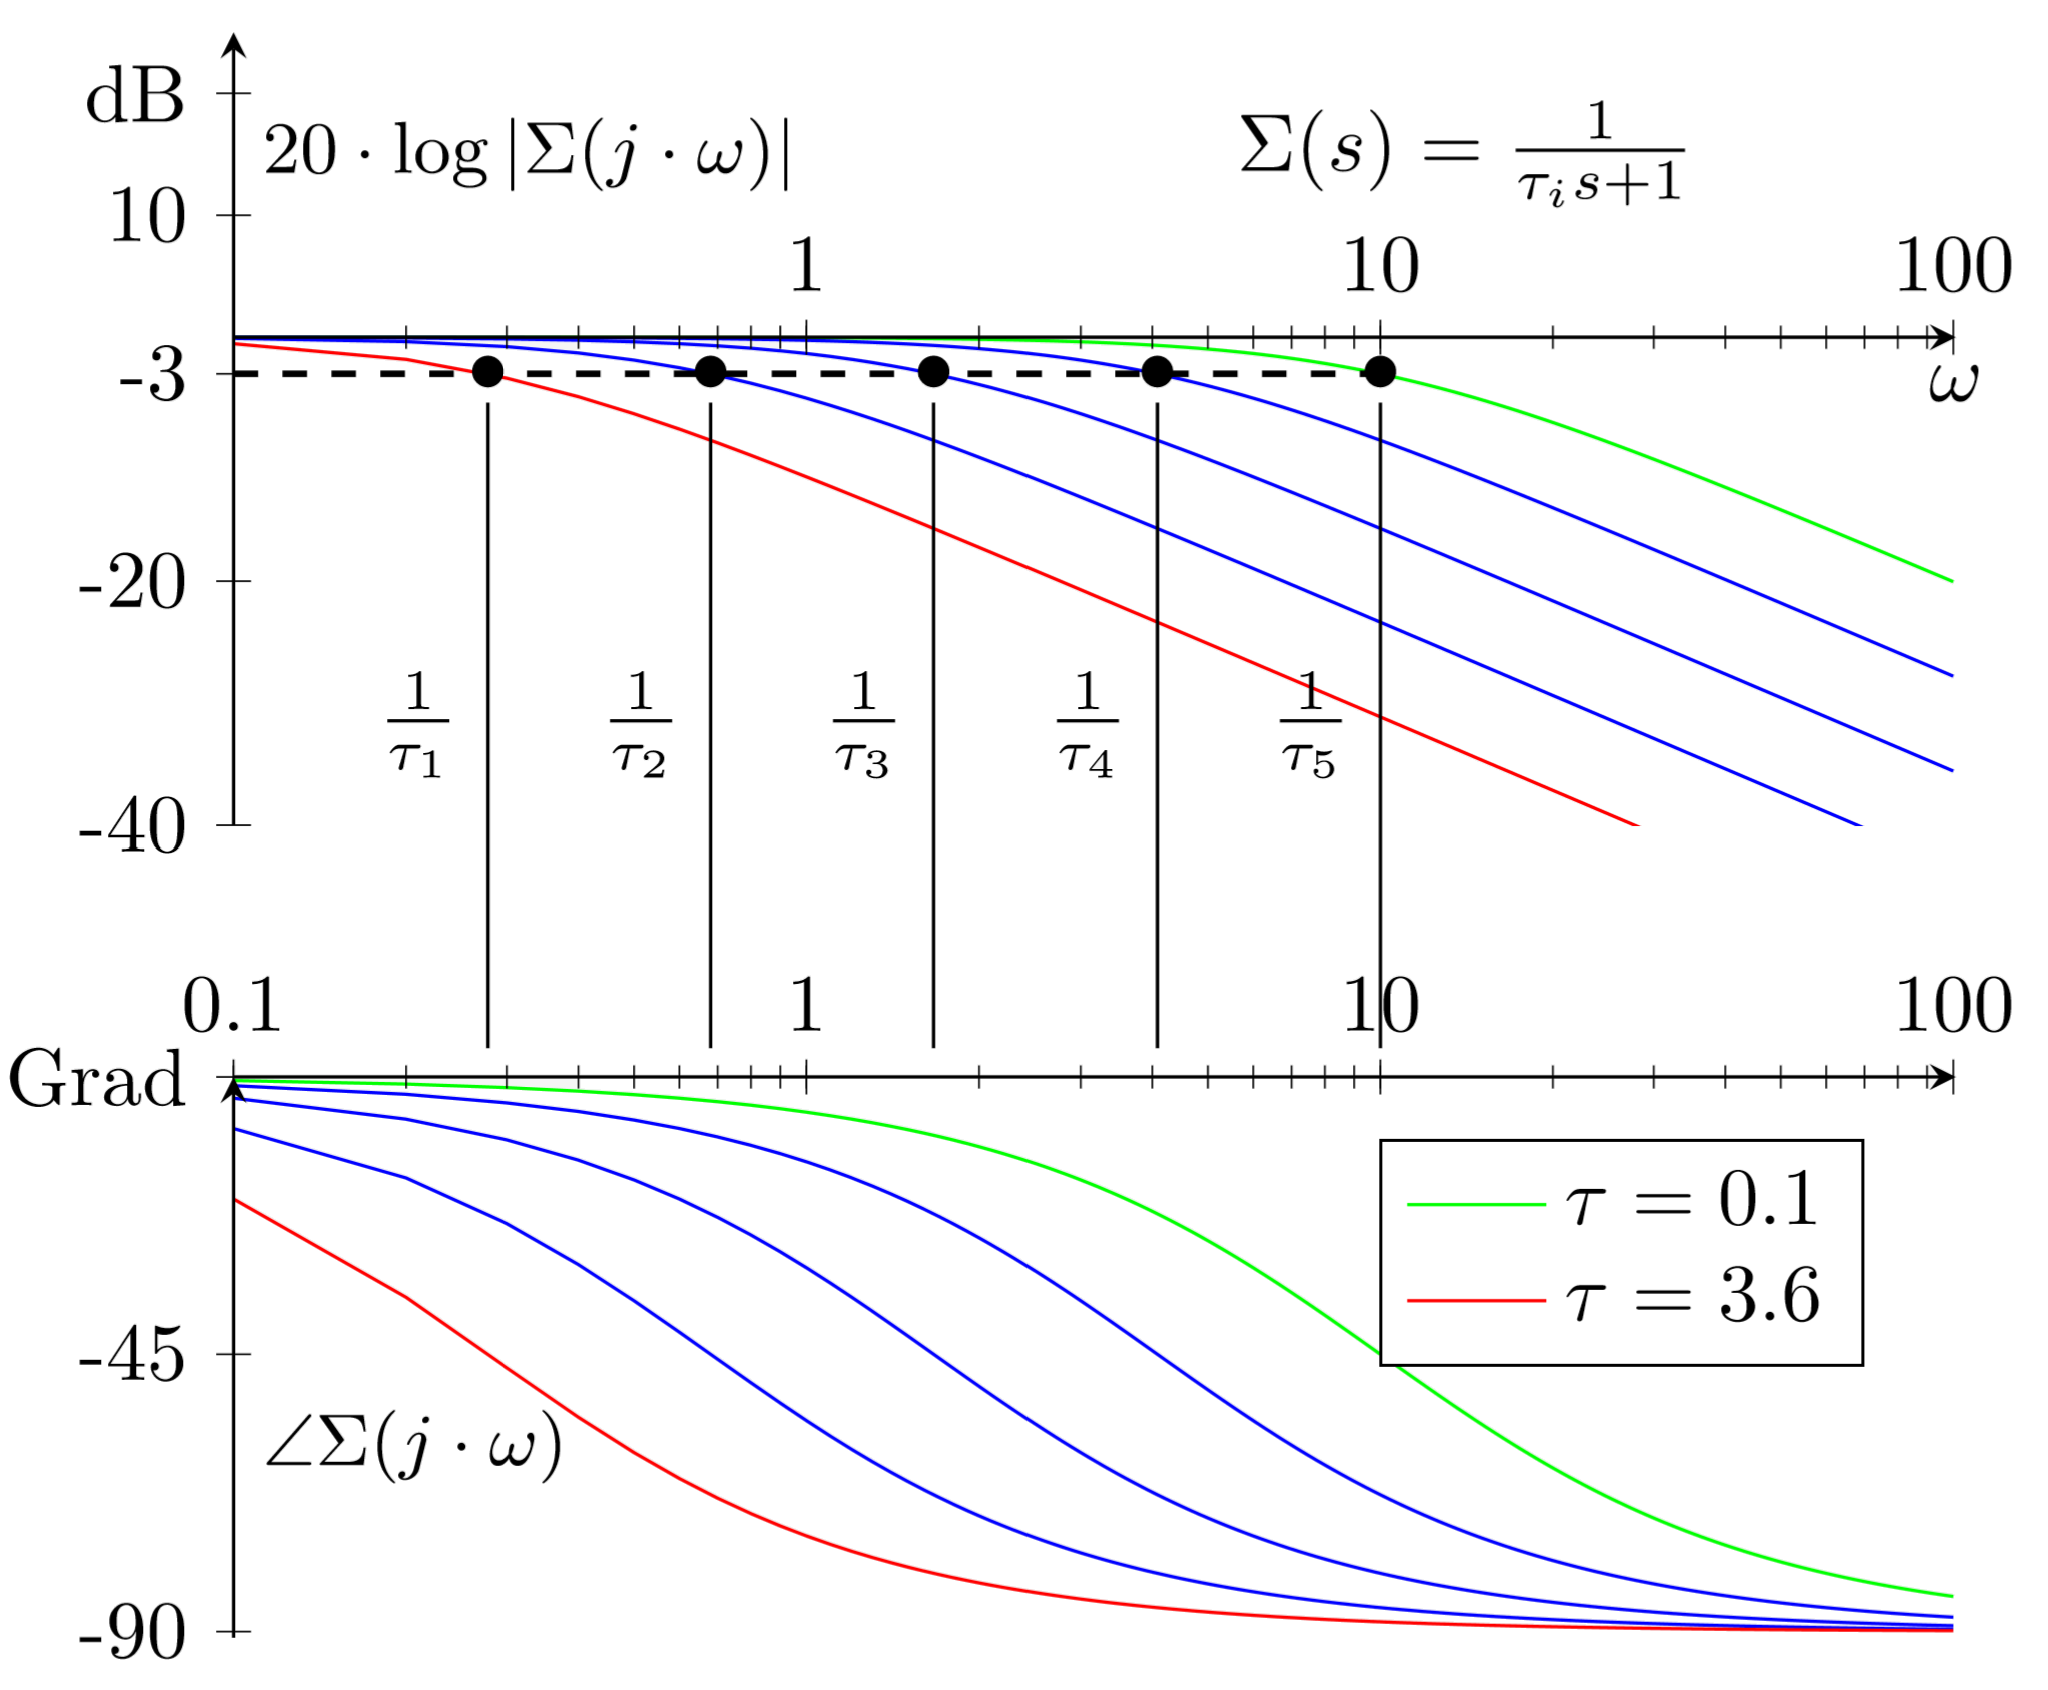
\includegraphics[width = 0.8\linewidth]{images/05/Bode_1Ordnung.png}
            \end{center}
        \subsubsection{Systeme 2. Ordnung}
            Viele mechanischen Systeme zeigen resonantes Verhalten (grössere Verstärkung bei mittleren Frequenzen als bei tiefen - eine sogenannte Resonanzüberhöhung). Solche Systeme werden oft als Systeme zweiter Ordnung approximiert.
            \begin{center}
                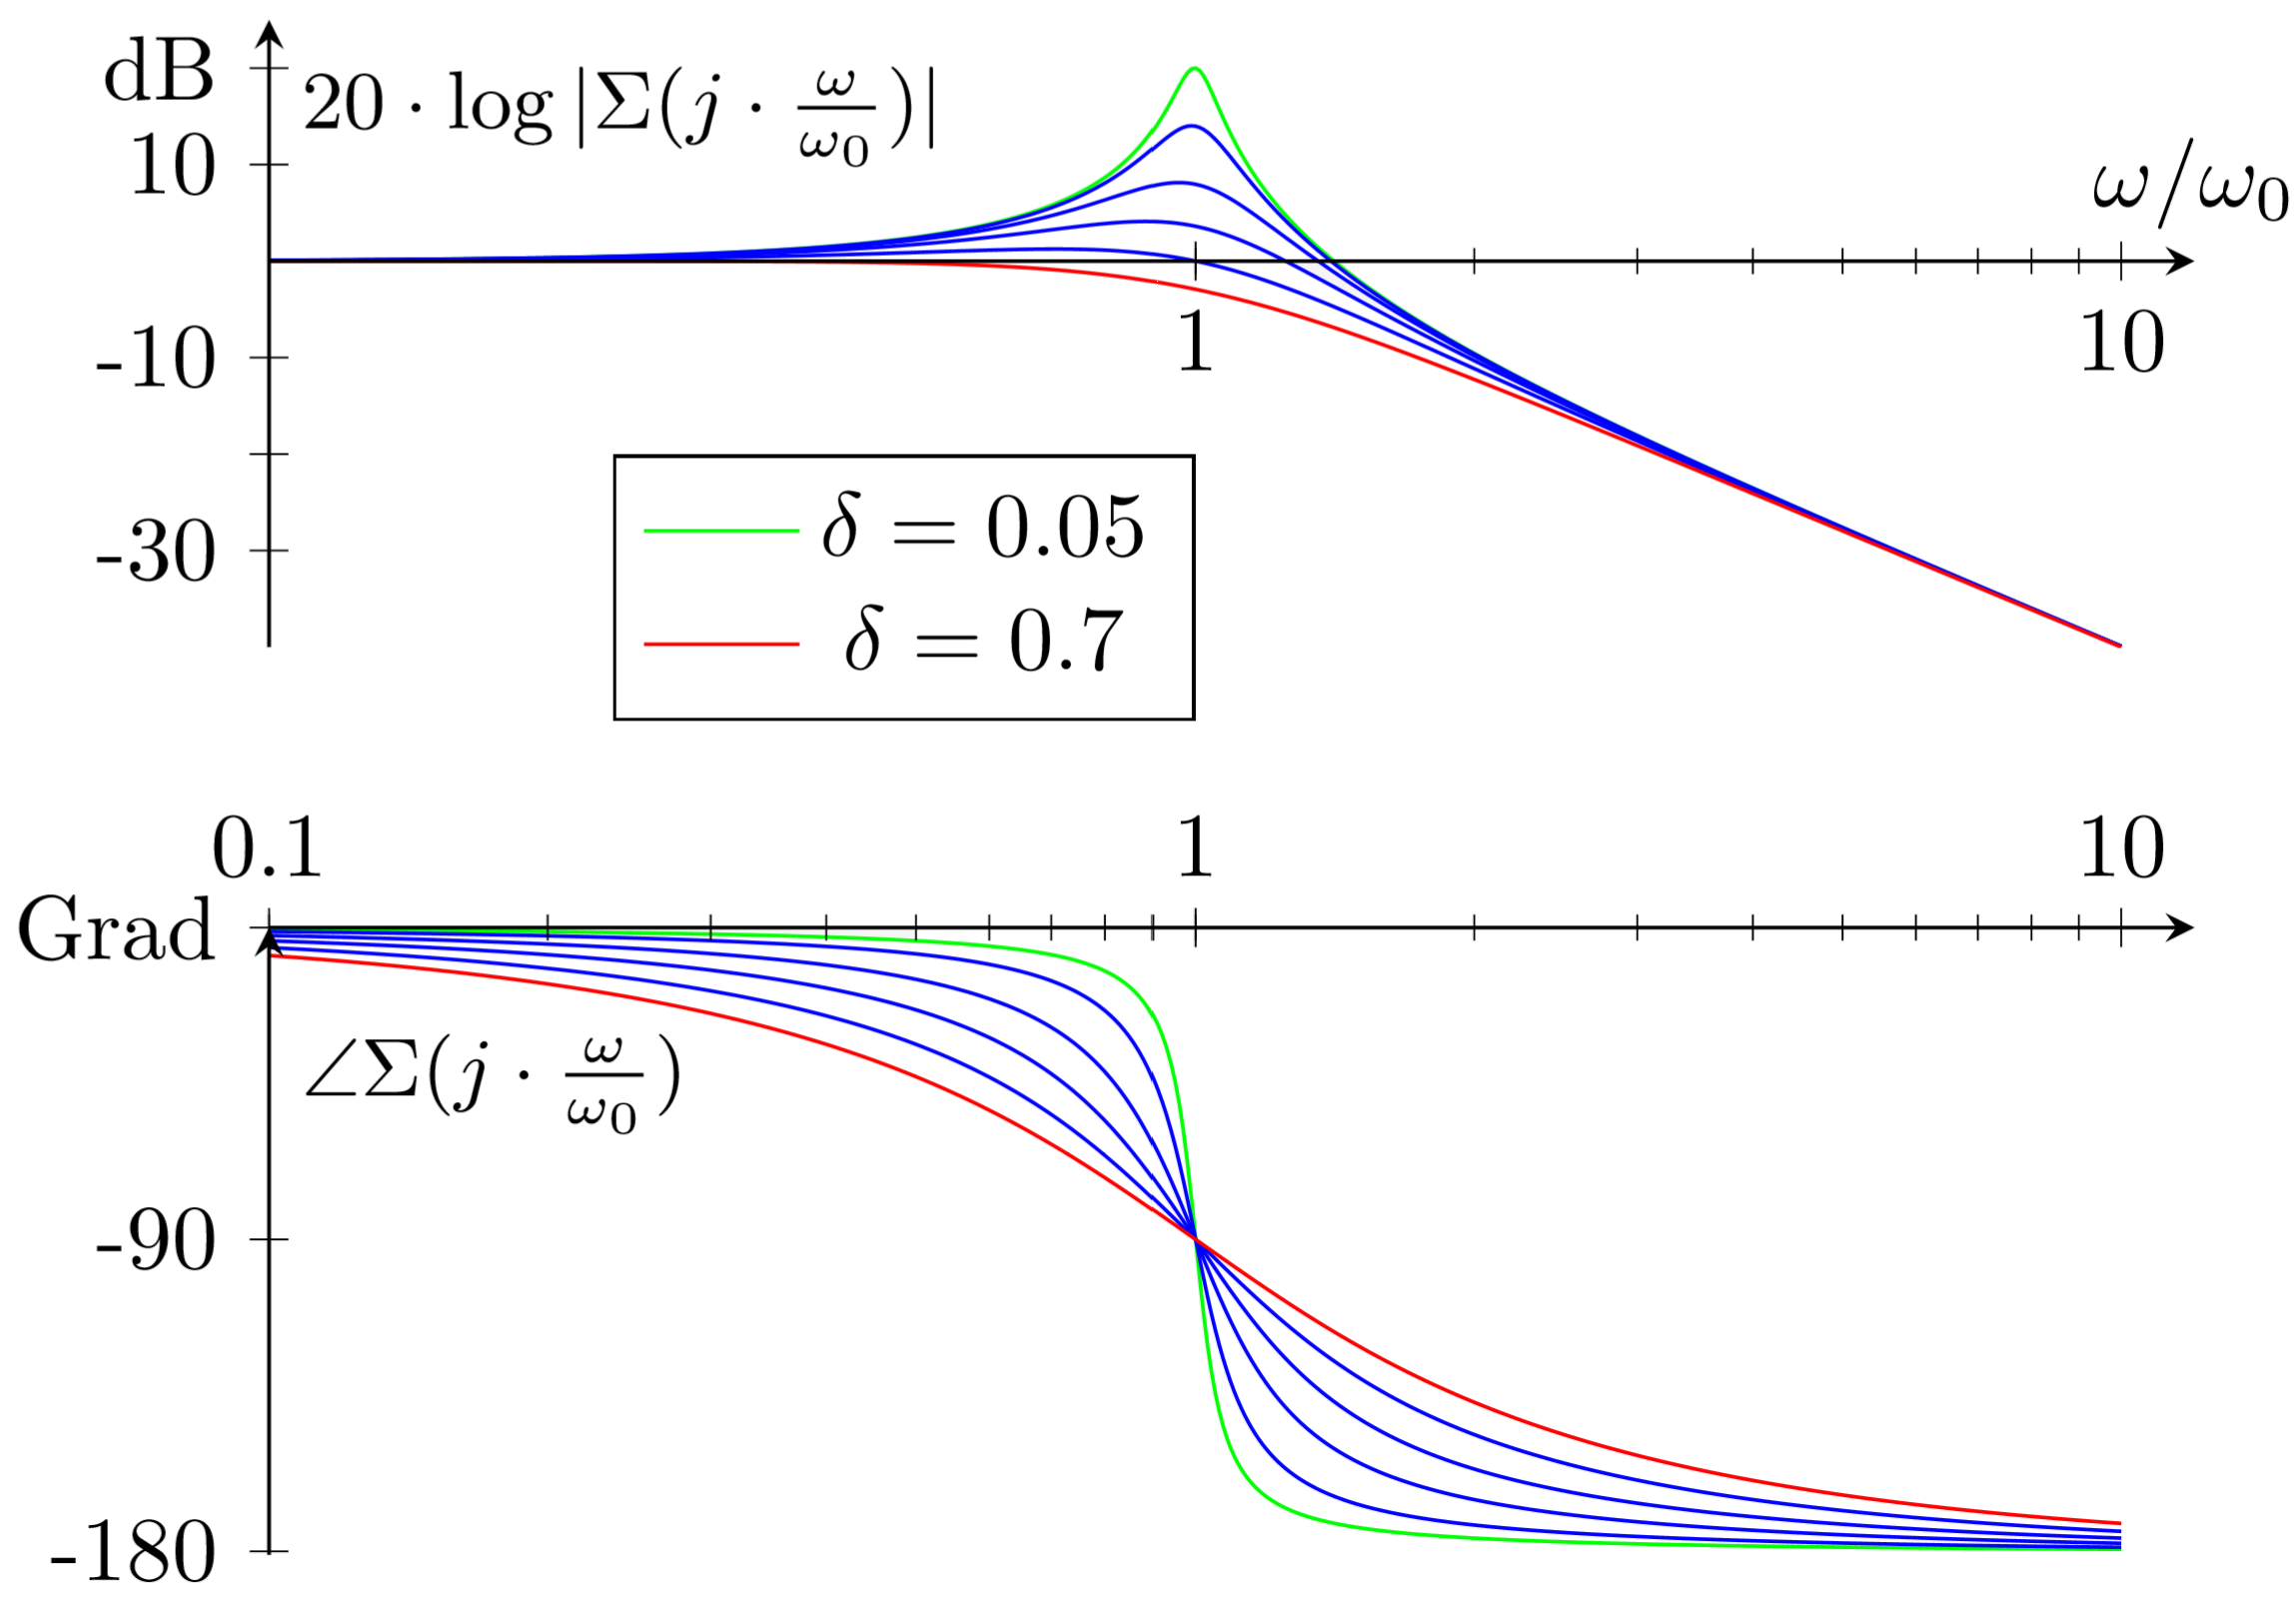
\includegraphics[width = 0.8\linewidth]{images/05/Bode_2Ordnung.png}
            \end{center}
            \textbf{Vorsicht!} Die resonante Frequenz (maximale Verstärkung) ist nicht bei der natürlichen Frequenz $\frac{\omega}{\omega_0} = 1$, sondern bei:
            \[\omega_{max} = \omega_0\cdot\sqrt{1-2\cdot\delta^2}, \hspace{4mm} 0<\delta<\frac{1}{\sqrt{2}}
            \]
            jedoch gilt für kleine Dämpfungsparameter $\omega_{max}\approx\omega_0.$ 
            Ausserdem zeigen Systeme 2. Ordnung für $\delta > \frac{1}{\sqrt{2}}$ kein resonantes Verhalten.
        \subsubsection{Einfluss von Polen \& Nullstellen auf das Bode Diagramm}
            {\renewcommand{\arraystretch}{1.4}
                \begin{tabular}{l|c|c}
                Standardelemente    &   Verstärkung $[\frac{dB}{dec}]$   &   Phase\\
                \hline
                Stabiler Pol    &   $-20$ bei $\omega_c$  &   $-90^{\circ}$ bei $\omega_c$\\
                Instabiler Pol    &   $-20$ bei $\omega_c$  &   $+90^{\circ}$ bei $\omega_c$\\
                Minimalphasige NST    &   $+20$ bei $\omega_c$  &   $+90^{\circ}$ bei $\omega_c$\\
                \small{Nichtminimalphasige NST}    &   $+20$ bei $\omega_c$  &   $-90^{\circ}$ bei $\omega_c$\\
                Delay um $\tau(\forall\omega)$ &    0   &   $-\frac{180}{\pi}\cdot\omega\cdot\tau^{\circ}$
            \end{tabular}}
    
        \subsubsection{Bsp}
            Zeichne Bode-Plot von $\Sigma(s)=\frac{100s}{(10s+1)(s+10)}$.
            \textbf{Vorgehen:}
            \begin{enumerate}
                \item In Standardelemente Zerlegen:
                \[\Sigma(s)=(100s)(\frac{1}{10s+1})(\frac{1}{s+10})\]
                \item NST/Pole der Standardelemente bestimmen:
                \[\zeta_1=0;\quad \pi_2=-\frac{1}{10};\quad\pi_3=-10\]
                \item Betrag der NST/Pole bestimmen.
                \[w_{\zeta}=|\zeta_1|=0;\quad w_{c_2}=|\pi_2|=\frac{1}{10};\quad w_{c_3}|\pi_3|=10\]
                \item $\Sigma(0)$ der einzelnen Elemente bestimmen.
                \[\Sigma_1(10^{-3})=0.1=-20dB;\quad \Sigma_2(0)=1=0dB;\]
                \vspace{-5mm}\[\Sigma_3(0)=\frac{1}{10}=-20dB\]
                \item Bode-Plot zeichnen 
            \end{enumerate}
            \begin{center}
                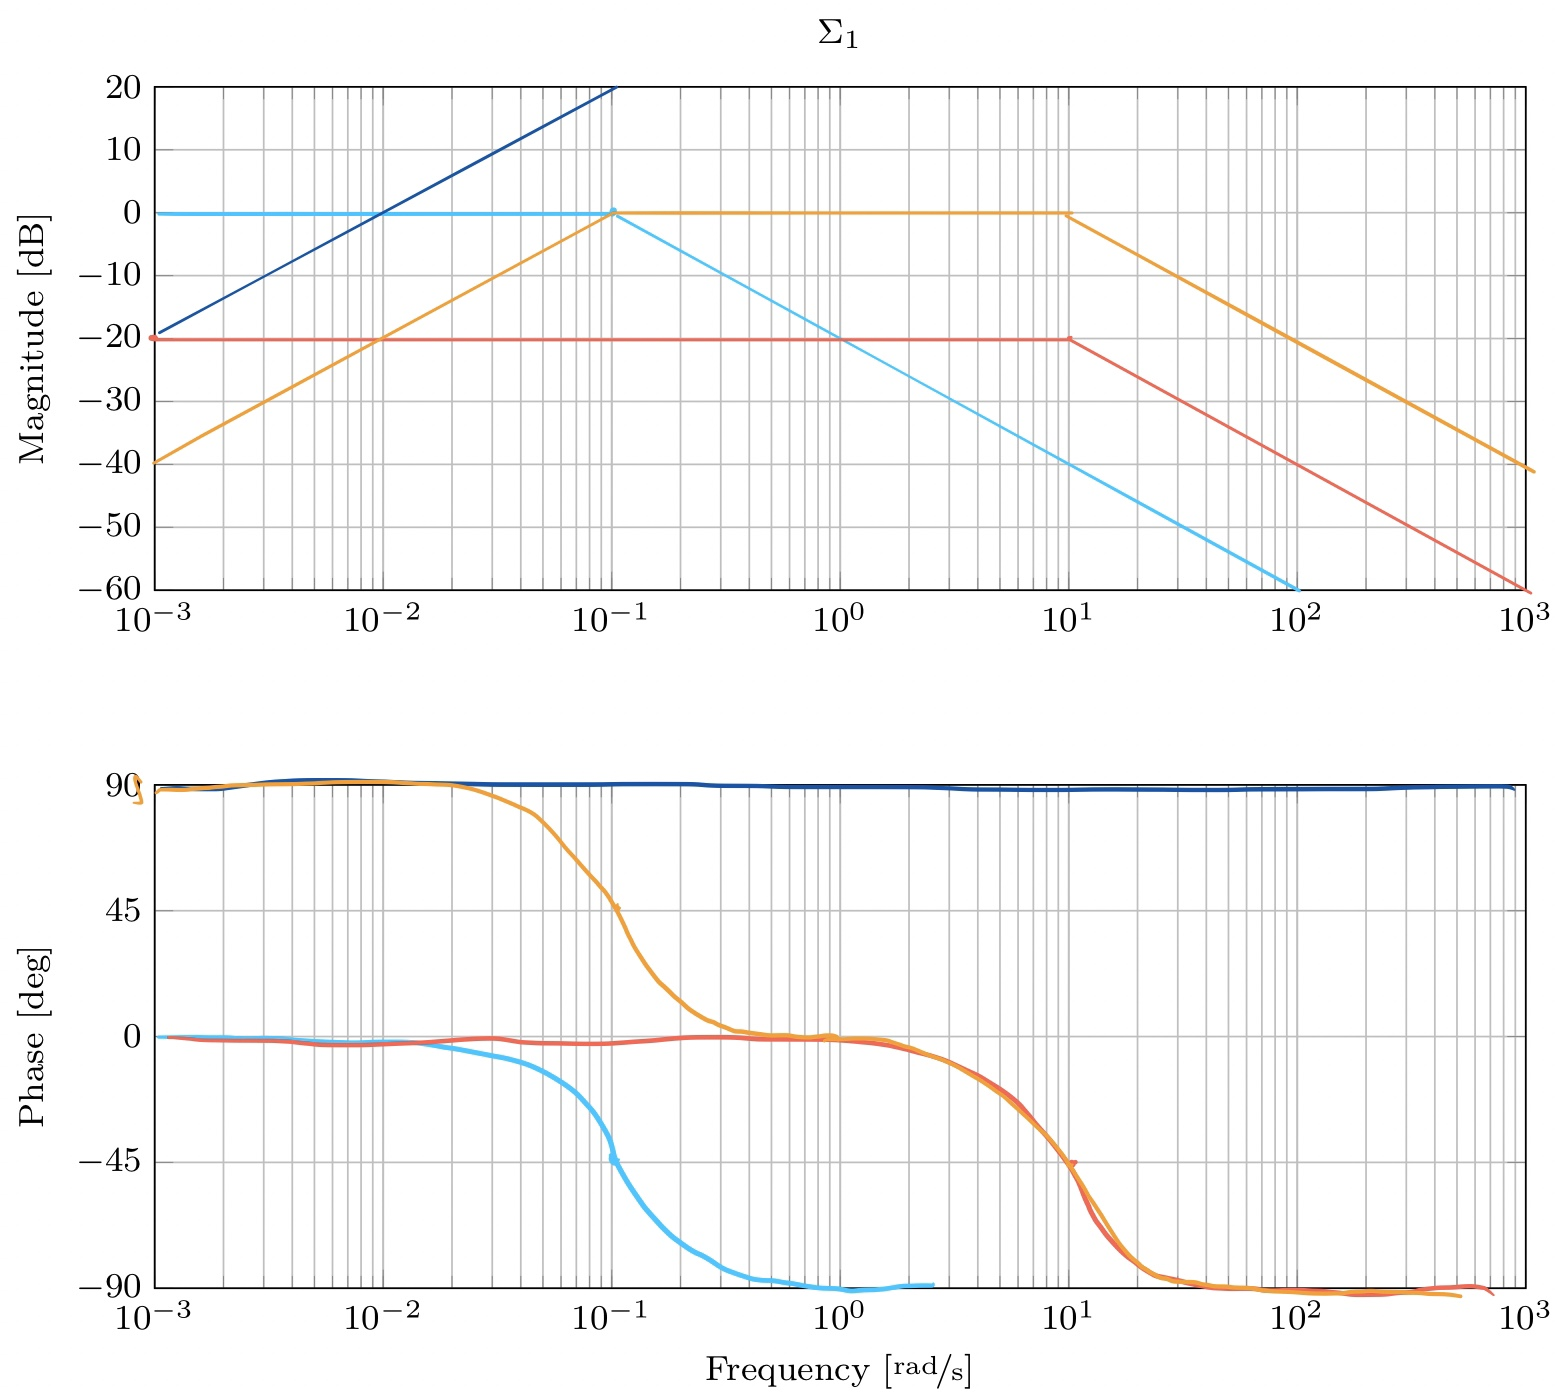
\includegraphics[width=0.6\linewidth]{05/bsp_bode.jpeg}
                \\\textit{Lösung in Orange}
            \end{center}
        \subsubsection{Bsp}
            Identifiziere Übertragungsfunktion in der From $\Sigma(s)=k\frac{s-\zeta}{s-\pi}$.
            \begin{center}
                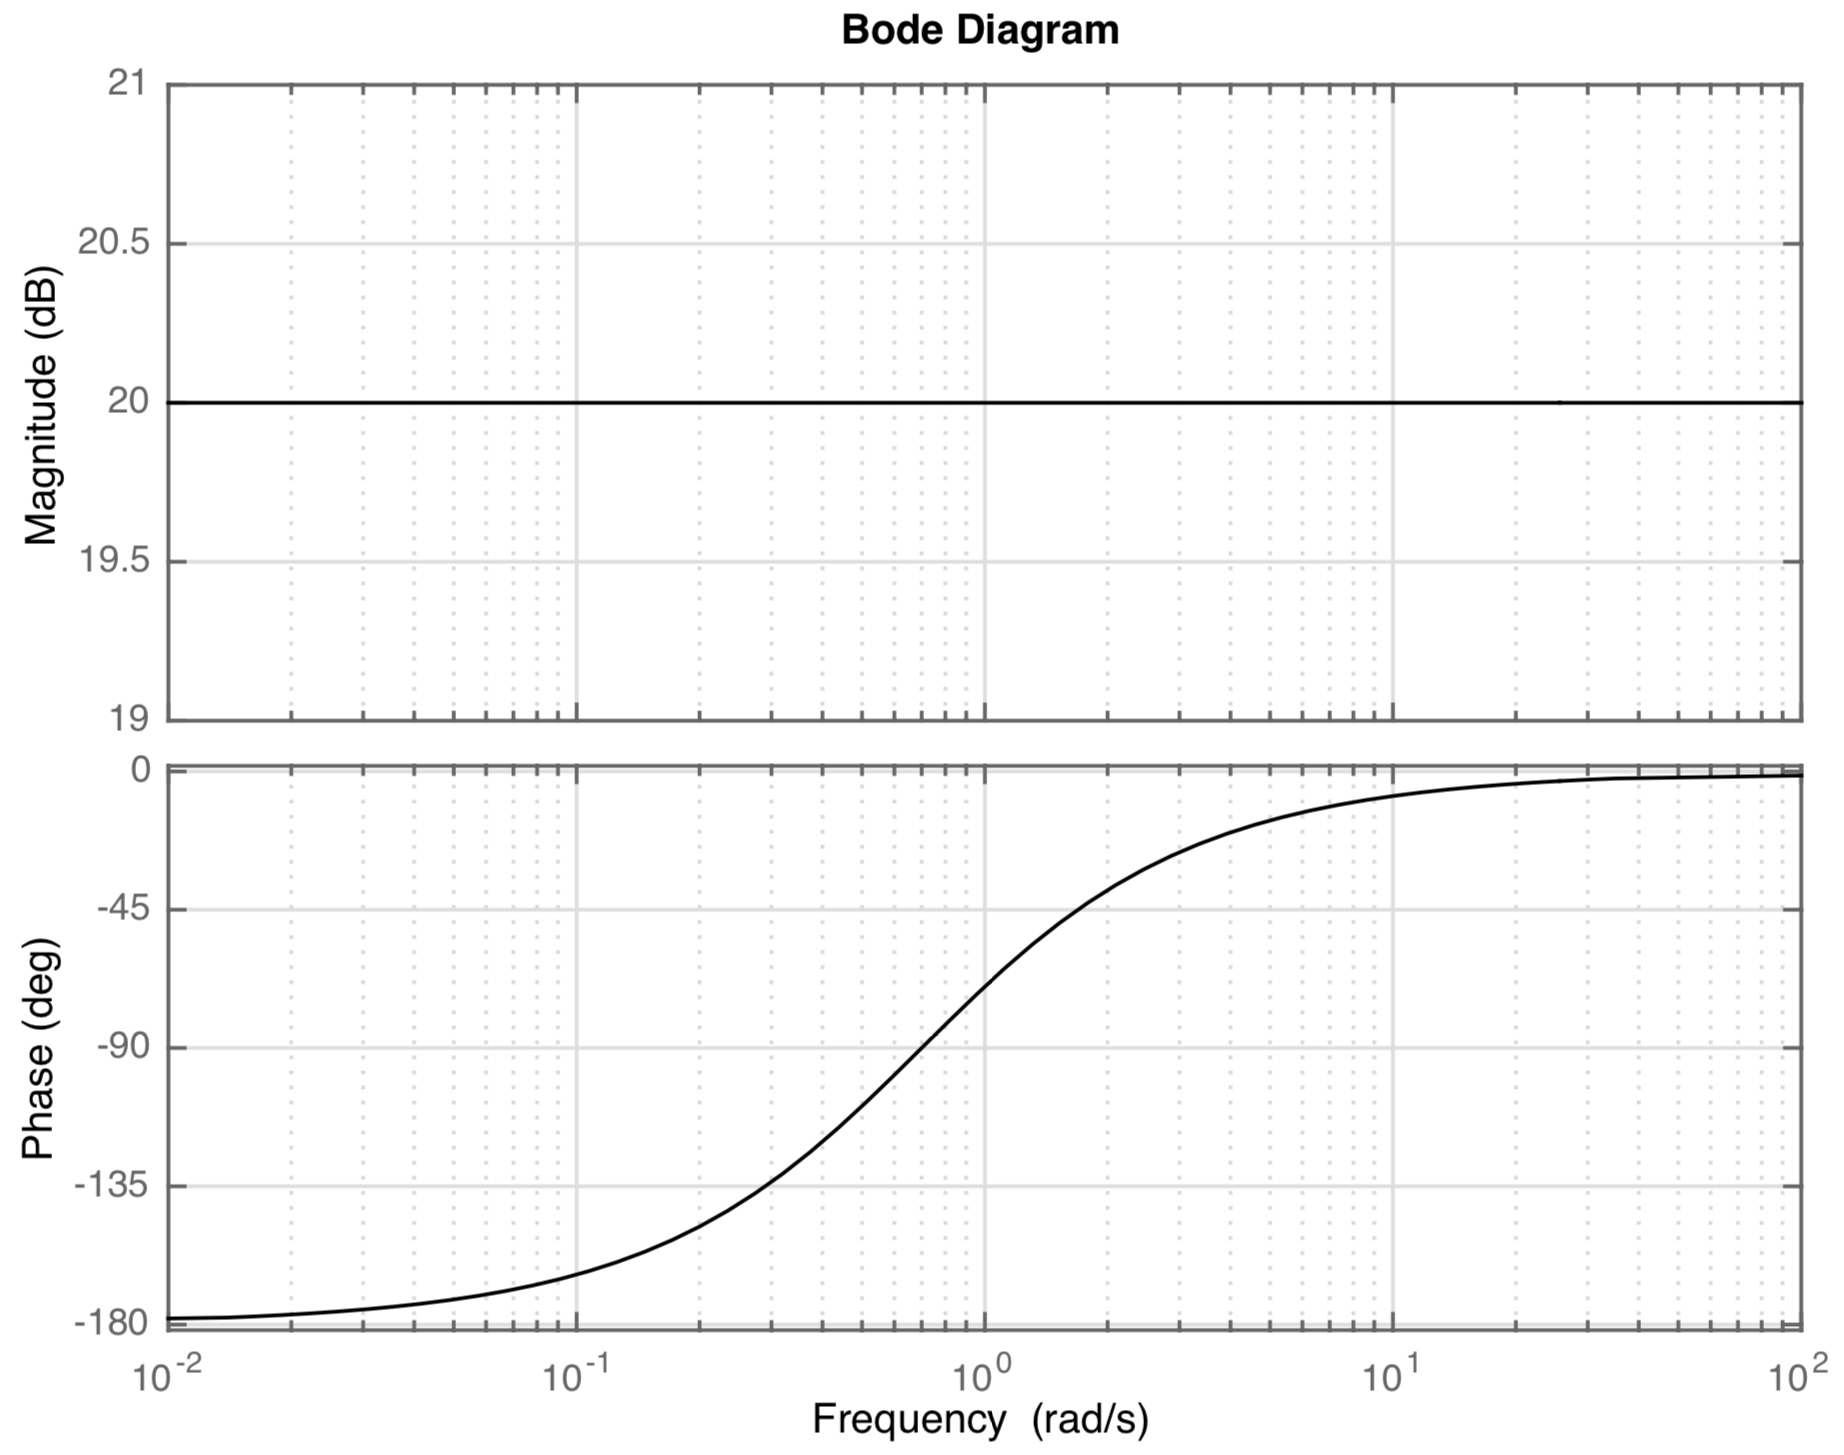
\includegraphics[width=0.47\linewidth]{05/neg_stat_gain.jpeg}
                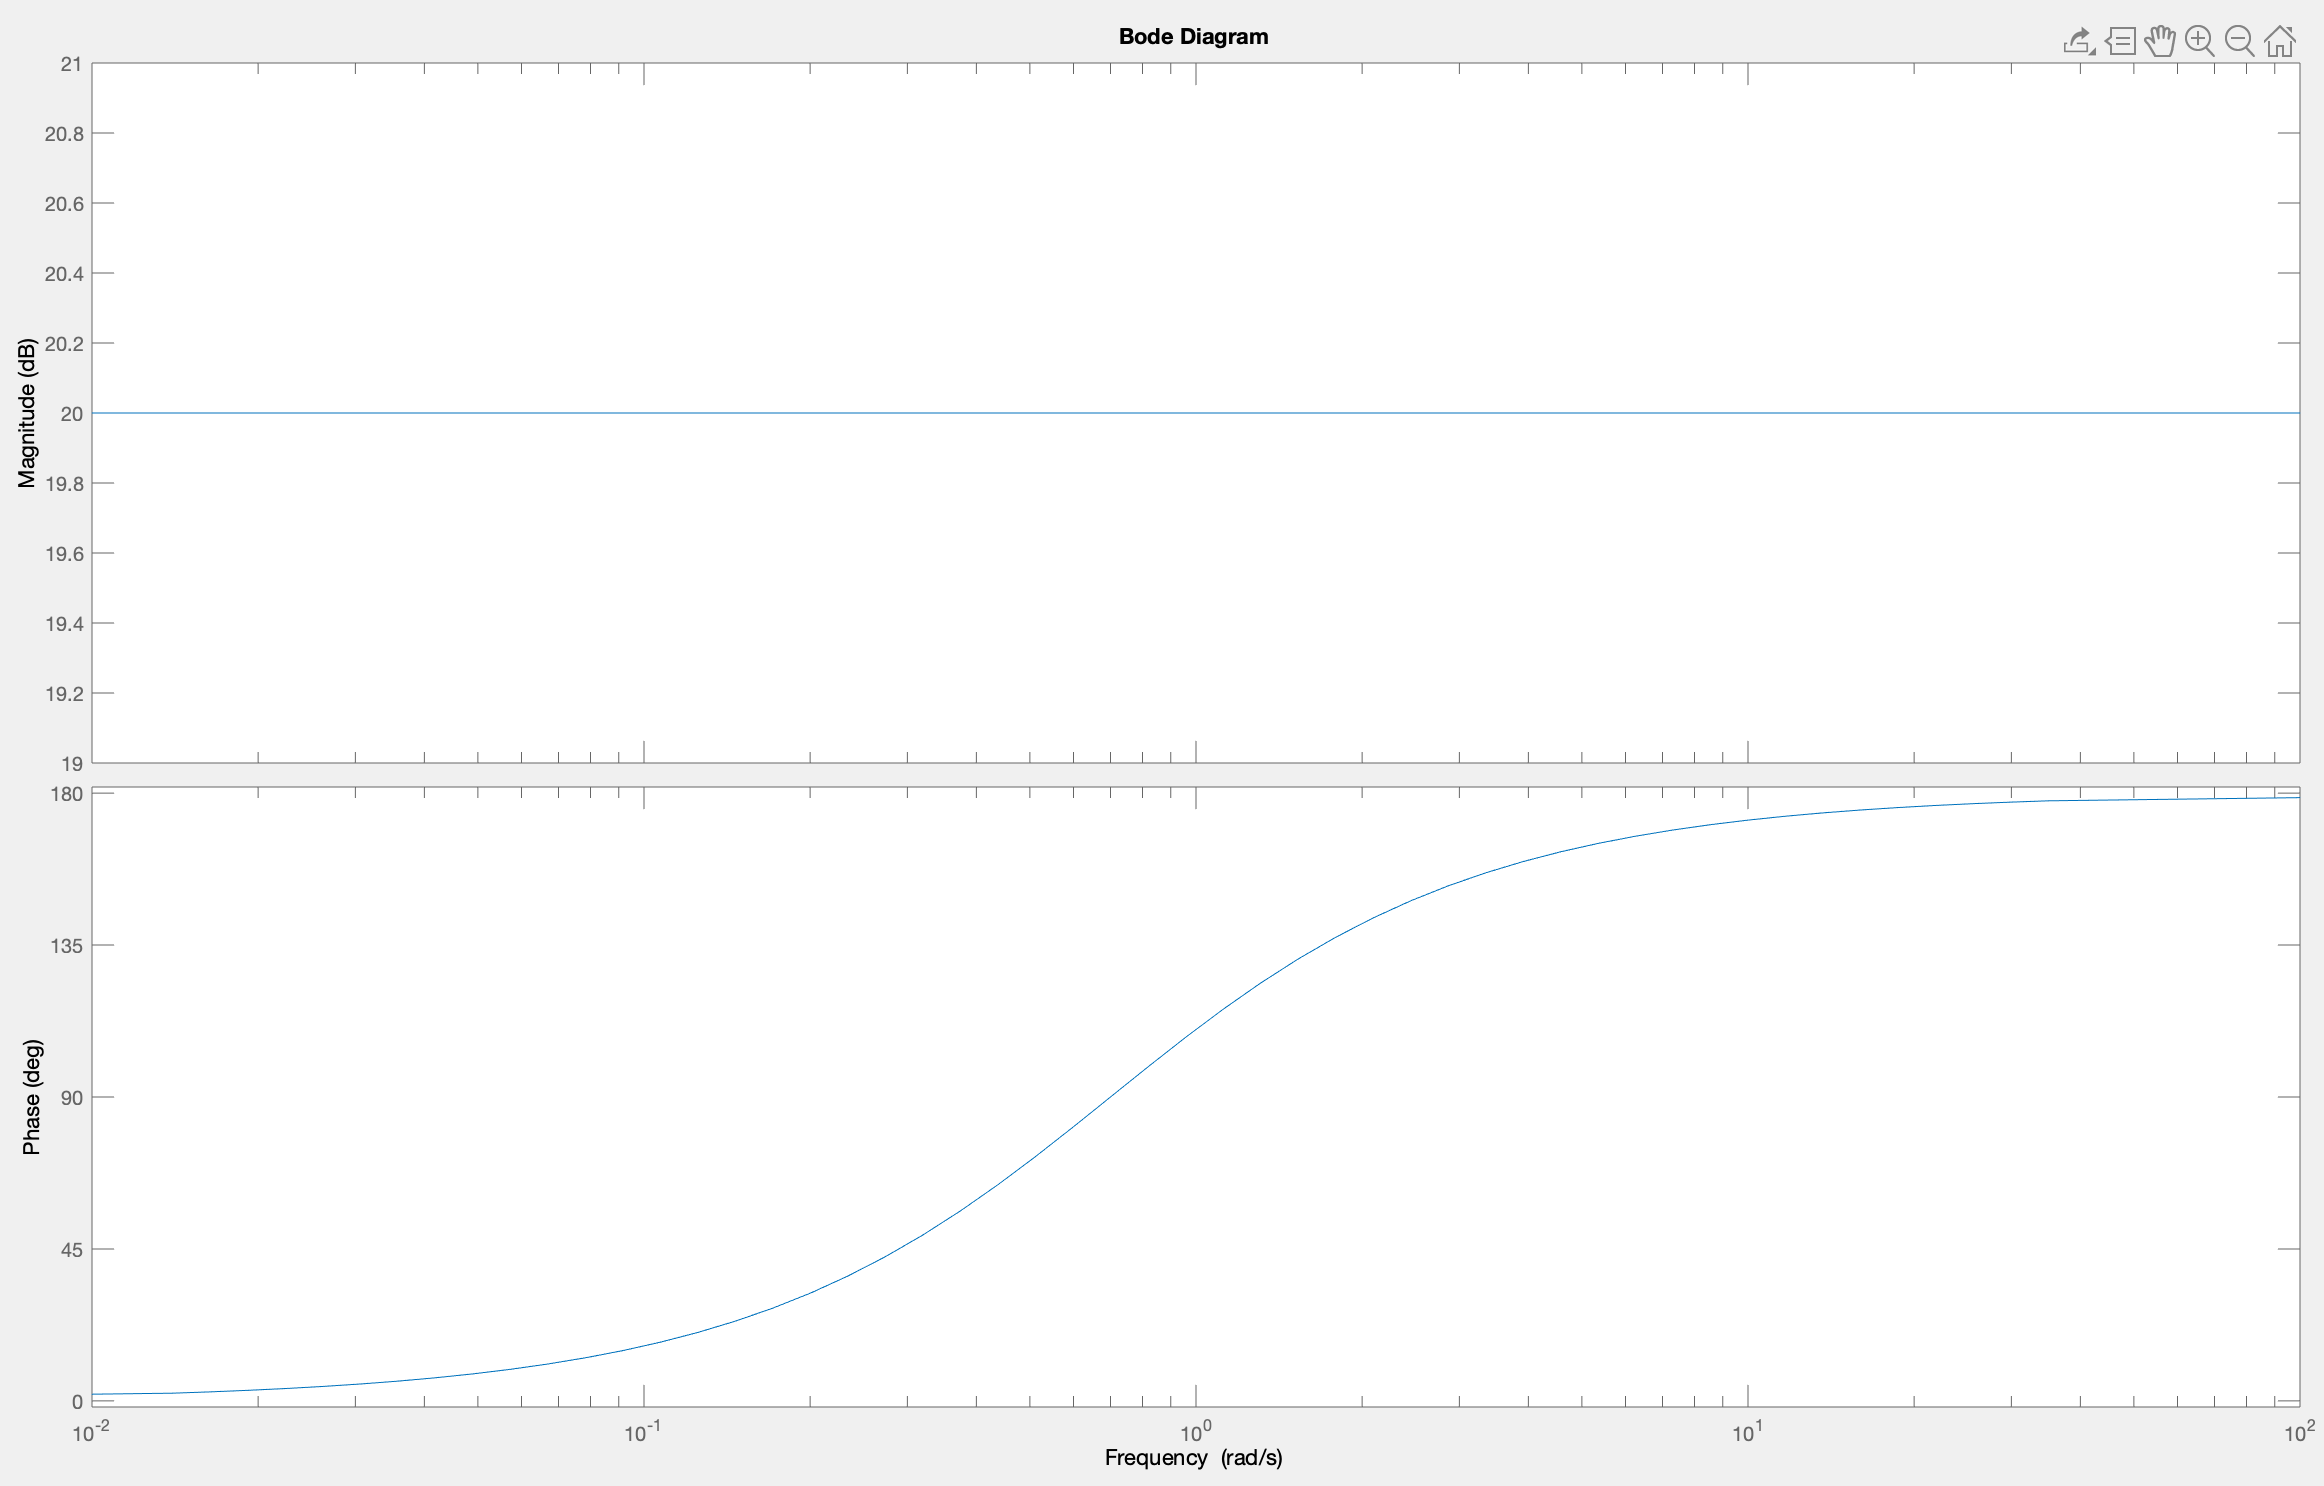
\includegraphics[width=0.5\linewidth]{images/05/neg_stat_gain_2.png}
                \small{\textit{Links: $\Sigma(s)$ mit negativer statischer Verstärkung}\\
                \textit{Rechts: $-1\cdot\Sigma(s)=:\Sigma(s)_{pos}$ mit positiver statischer Verstärkung}}
            \end{center}
            \begin{enumerate}
                \item $|\Sigma(s)|=20dB \quad\forall\omega$ $\rightarrow$ Pol und Nullstelle müssen an der selben Stelle sein. Da das System eine neg. stat. Verstärkung hat rechnen wir das gesamte System mal $-1$. Dadurch gewinnt das System $180^{\circ}$ Phase. So können wir das System aus Standardelementen darstellen.
                \item System gewinnt an $180^{\circ}$ Phase $\rightarrow$ eine stabile NST und ein instabiler Pol.
                \item Auslesen aus Bode Plot ergibt für $|\pi|=|\zeta|=0.7$ und $|\Sigma(s)_{pos}|=k\frac{\sqrt{\omega^2+0.7^2}}{\sqrt{\omega^2+0.7^2}} \Rightarrow k=20dB=10$
                \item $\Sigma(s)_{pos}=-10\frac{s+0.7}{s-0.7} \Leftrightarrow \Sigma(s)=10\frac{s+0.7}{s-0.7}$
            \end{enumerate}
                \begin{center}
                    \textbf{Falls Anzahl mini-phasige NST + instabile Pole \textit{ungerade}, hat das System neg. stat. Verstärkung}
                \end{center}
                
                
    \subsection{Nyquist Diagramme}
        Darstellung des Frequenzganges (Magnitude und Phase über die Anregungsfrequenz $\omega$) in der komplexen Ebene.
        \subsubsection{Systeme 1. Ordnung}
        Ein allgemeines System 1. Ordnung bei der Frequenz $s= j\omega$ hat folgende Magnituden und Phasen, wobei $\tau = \frac{1}{\omega_c} $:
        \[|\Sigma(j\omega)| = \frac{1}{\sqrt{\tau^2\omega^2+1}}
        \qquad
        \angle\Sigma(j\omega) = -arctan(\tau\cdot\omega)
         \]
        \begin{center}
        \vspace{-2mm}
            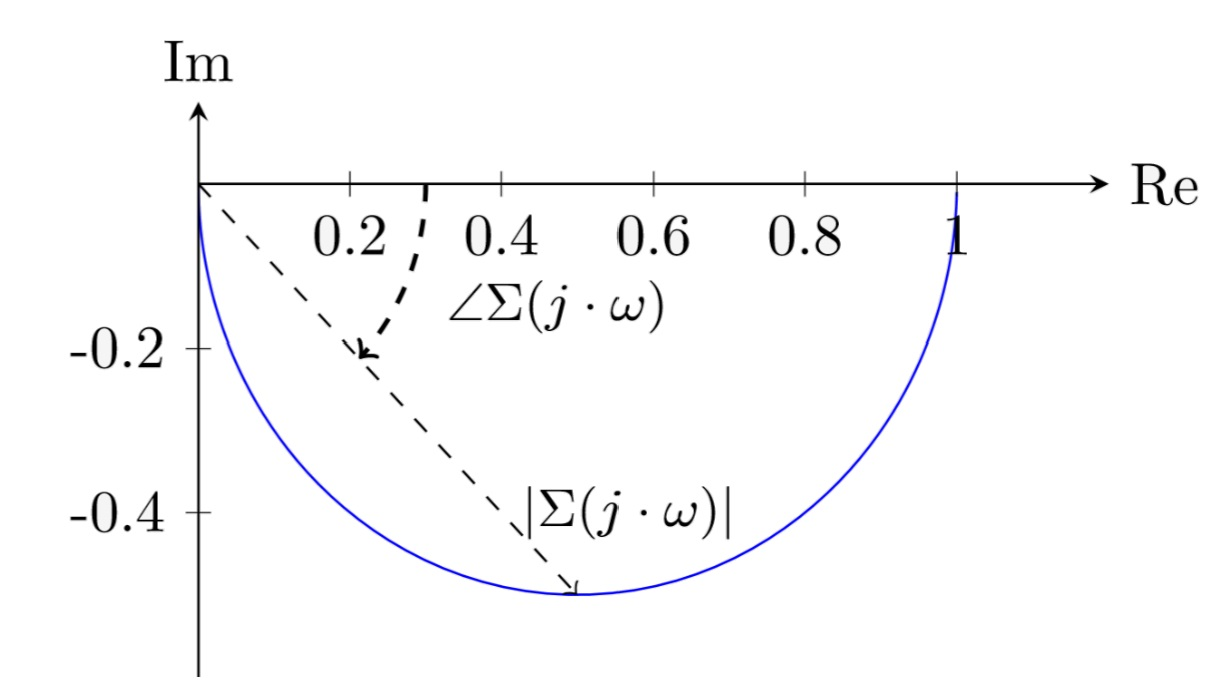
\includegraphics[width=0.6\linewidth ]{images/05/Nyq_1Ordnung.jpg}
        \end{center}
        \textbf{Bemerkung:} Für alles Systeme 1. Ordnung $\displaystyle\Sigma(s)=\frac{k}{T\cdot s+1}$ mit $\omega\in(-\infty,\infty)$ ist die Nyquist-Kurve ein Kreis mit Mittelpunkt $(k/2,0)$.
    
        \subsubsection{Systeme 2. Ordnung}
            Ein allgemeines System 2. Ordnung hat bei der Frequenz $s=j\cdot\omega$ folgende Magnituden und Phasen:
            \[ |\Sigma(j\omega)| = \frac{\omega_0^2}{\sqrt{(\omega_0^2-\omega^2)^2+4\cdot \delta^2 \cdot \omega_0^2\cdot \omega^2}}\]
            \[
            \angle\Sigma(j\omega) = \begin{cases} -arctan(\dfrac{2\cdot\delta\cdot\omega_0\cdot\omega}{\omega_0^2-\omega^2}) & \forall 0 \leq \omega \leq\omega_0 \\
            \\  
            -arctan(\dfrac{2\cdot\delta\cdot\omega_0\cdot\omega}{\omega_0^2-\omega^2}) -\pi & \forall \omega_0 < \omega
            
            \end{cases}
            \]
            \begin{center}
                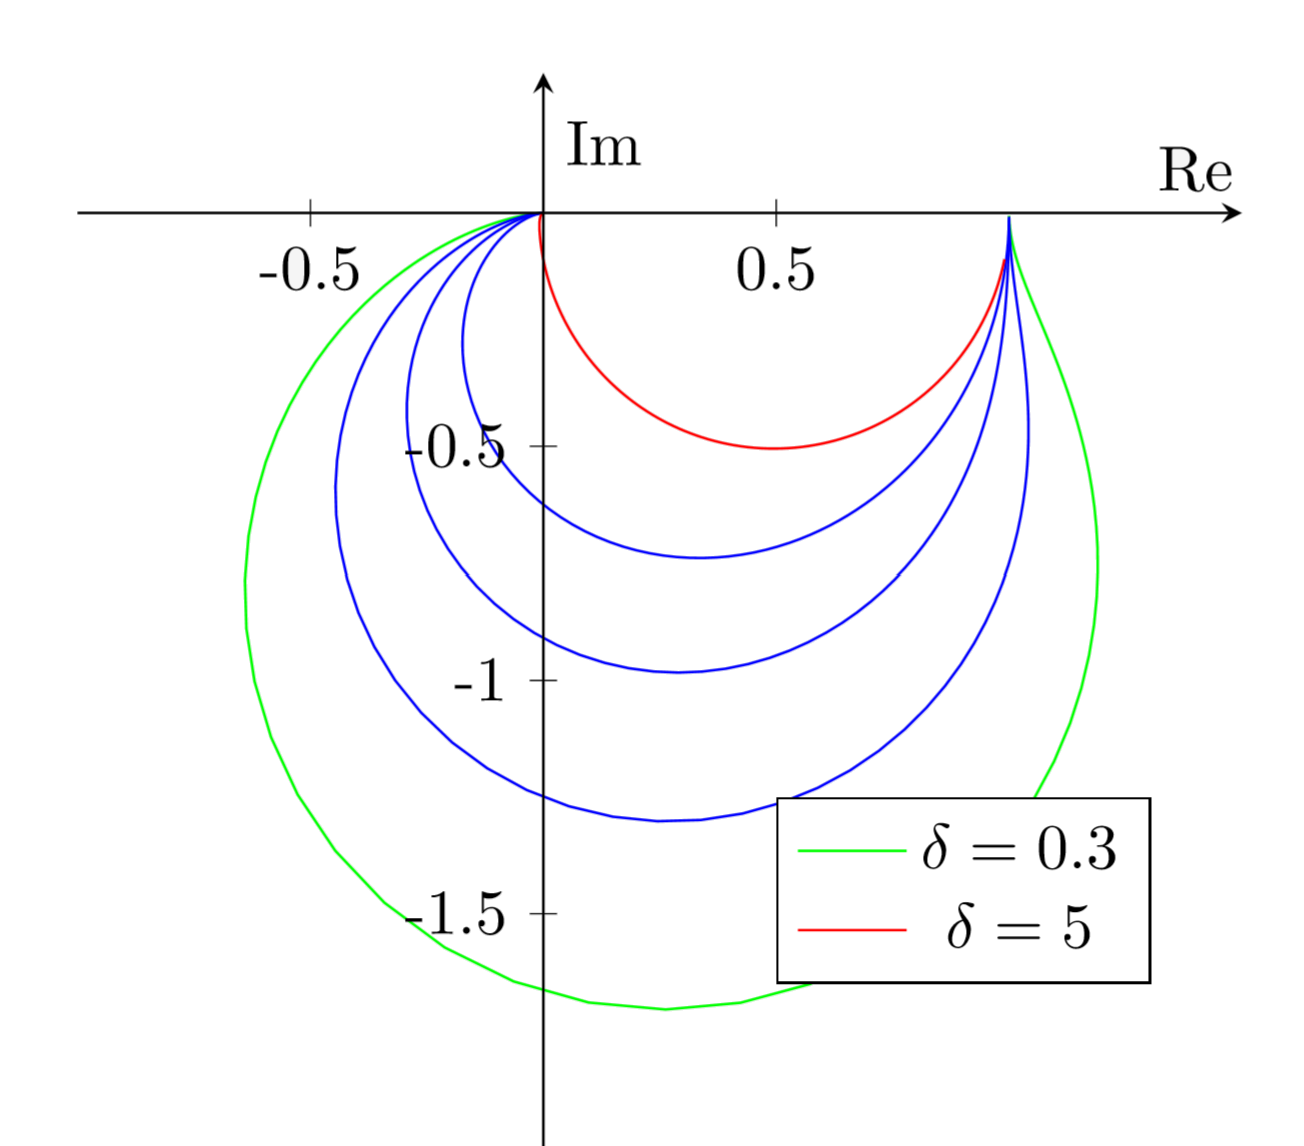
\includegraphics[width = 0.5\linewidth]{images/05/Nyq_2Ordnung.jpg}
            \end{center}

        \subsubsection{Bsp}
            Gegeben sei eine Kreisverstärkung $\frac{1}{s^2+s+1}$
            man will $\angle L(j\omega)$ für $\omega \rightarrow \infty$ herausfinden.
            \textbf{Achtung!} nicht einfach einsetzten und ausmultiplizieren! stattdessen zwei Nullststellen ausfindig machen und dann einsetzen. 
            
            \textbf{Für sehr hohe Frequenzen gilt:}
            \begin{center}
                \renewcommand{\arraystretch}{1.3}{\begin{tabular}{l|c}
                  offener Integrator $\frac{1}{s^k}$   & $\displaystyle\lim_{\omega\to\infty}\angle L(j\omega)= -k\cdot \frac{\pi}{2}$ \\
                   \#instabiler Pol   & \#$+\frac{\pi}{2}$ \\
                   \#stabiler Pol & \#$-\frac{\pi}{2}$\\
                   \#minimalphasige Nullstelle &   \#$+\frac{\pi}{2}$\\
                   \#Nicht-minimalphasige Nullstelle & \#$-\frac{\pi}{2}$
                \end{tabular}}
            \end{center}
        
         \subsubsection{Bsp}
            \begin{center}
                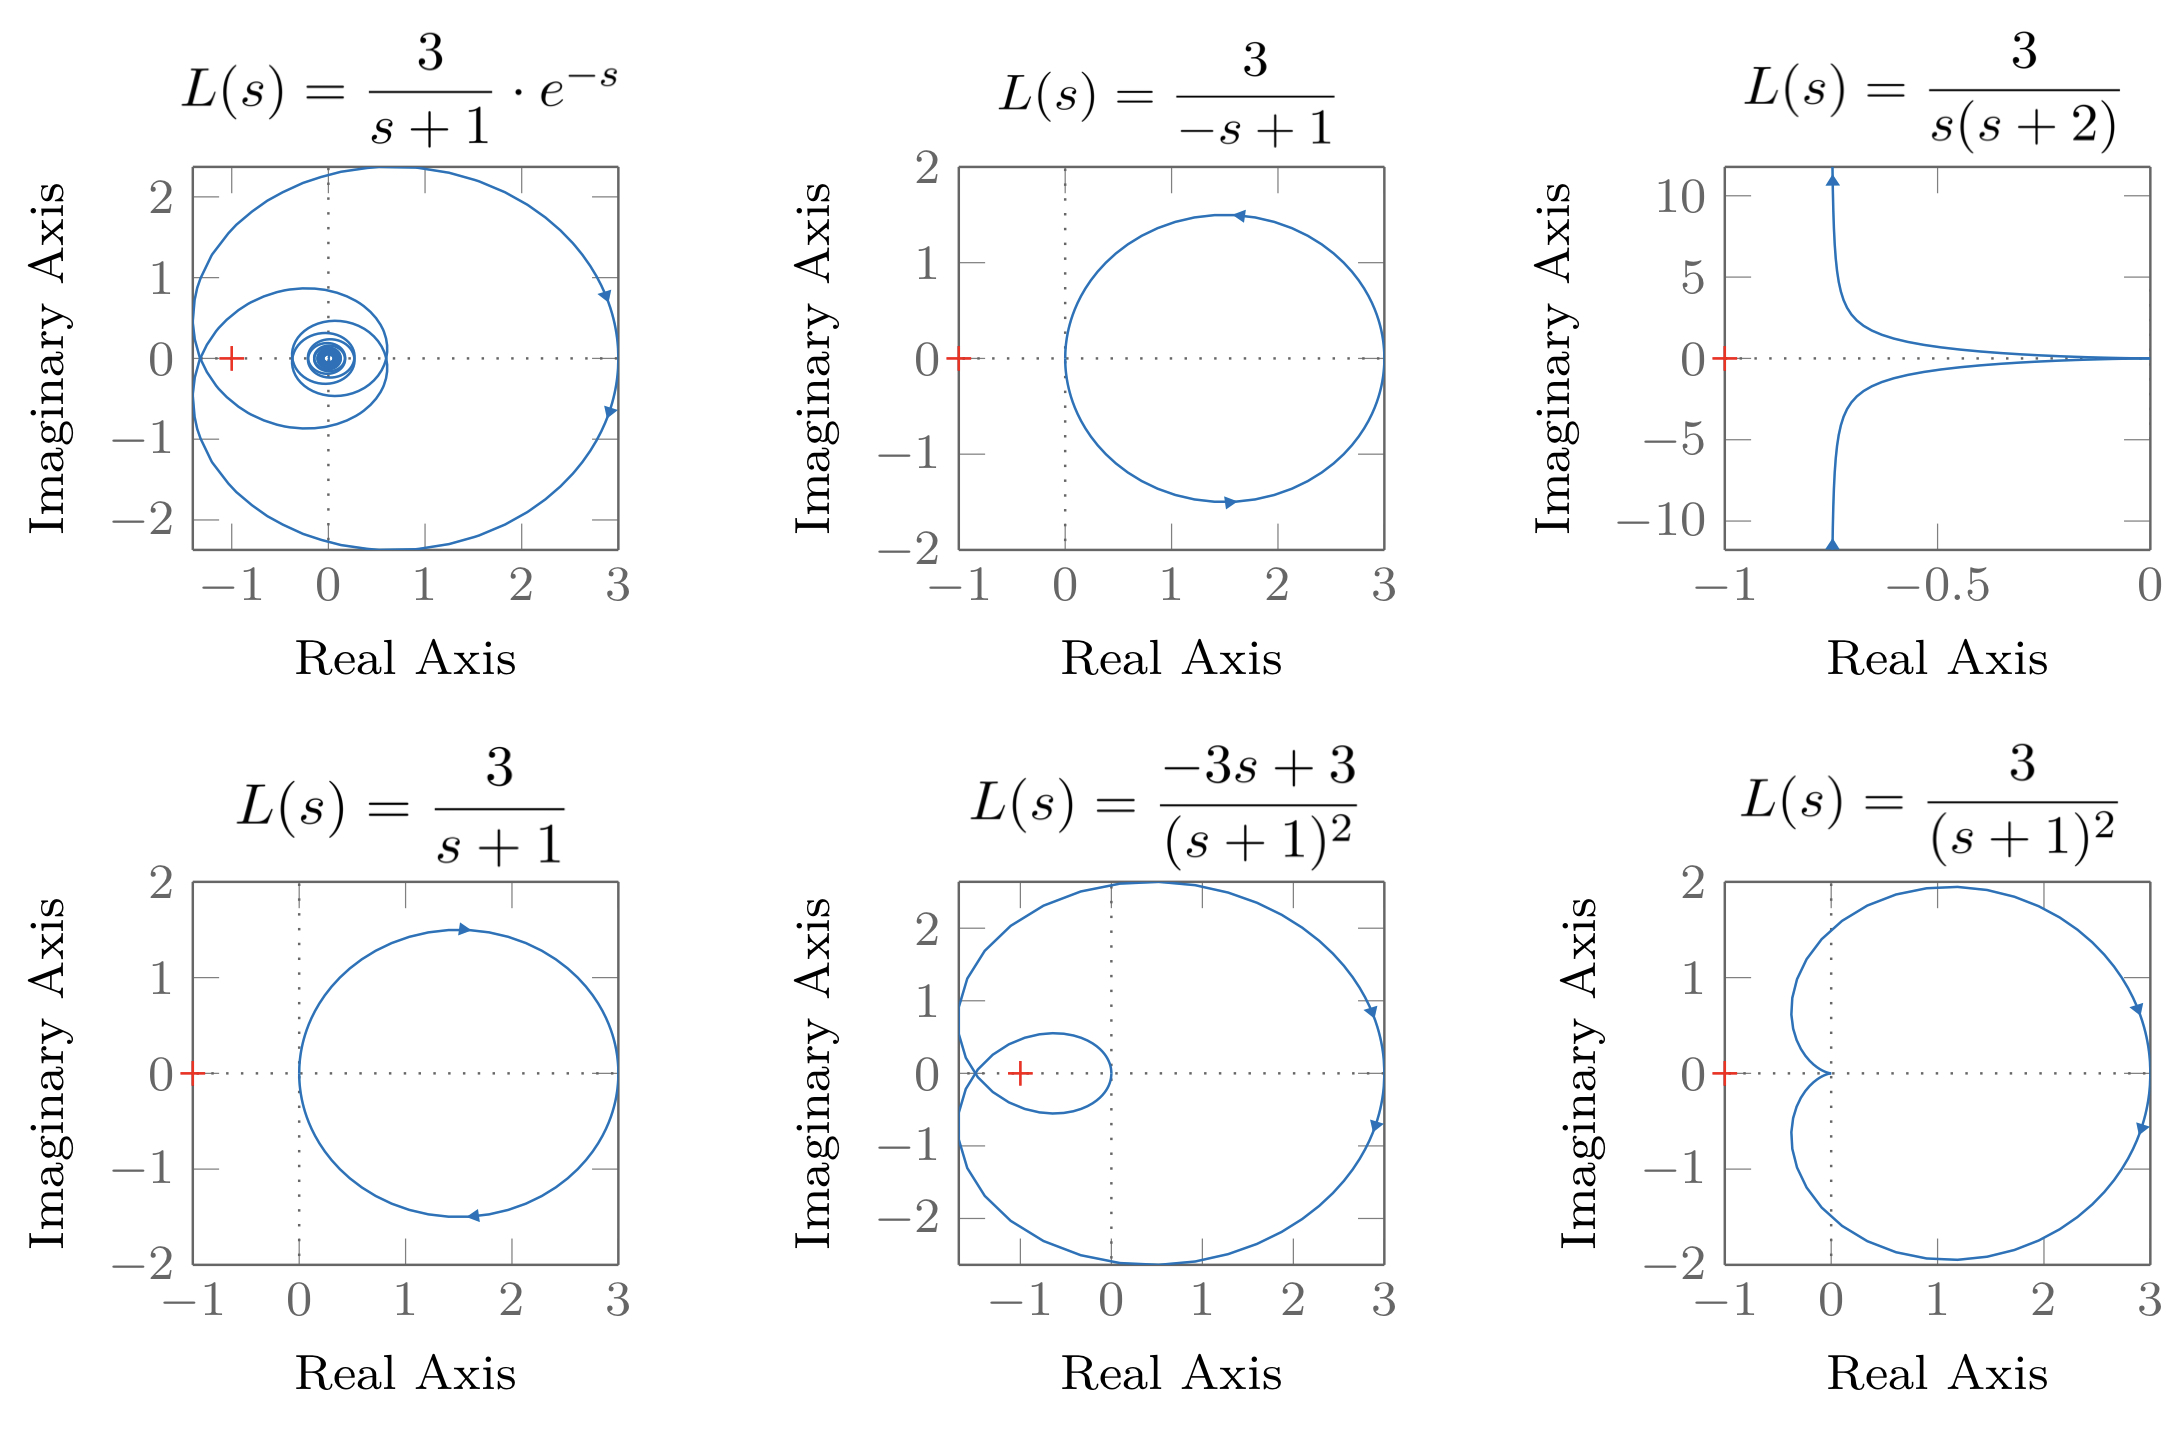
\includegraphics[width=\linewidth]{images/05/bsp_nyquist.jpeg}
                \textit{Einige Übertragungsfunktionen und ihre Nyquist-Diagramme}
            \end{center}
            
    \subsection{Asymptotische Eigenschaften von Frequenzantworten}
        Gegeben sei die folgender Struktur einer allgemeinen Übertragungsfunktion:
        \[\Sigma(s) = \frac{b_m\cdot s^{\mathbf{m}}+\hdots + b_1 \cdot s + b_0}{s^{\mathbf{k}}\cdot (s^{\mathbf{n}-k}+a_{n-1-k}\cdot s^{n-1-k}+\hdots+ a_1 \cdot s + a_0)}\]
        Aus der Übertragungsfunktion kann man direkt die \textbf{Phase} bei $\omega = 0$ aus dem \textbf{Systemtyp} $k$ bestimmen. 
        Zusätzlich kann man das Asymptotische Verhalten der Magnitude $|\Sigma(j\omega)|$ für $\omega \rightarrow \infty$ direkt aus dem \textbf{relativen Grad} $ r=n-m$ bestimmen.
        
        \subsubsection{Systemtyp $k$}
        Der \textbf{Systemtyp $k$} entspricht der Vielfachheit offener Integratoren $\frac{1}{s^k}$ des Systems. Die Phase bei $\omega = 0$ lässt sich folgendermassen bestimmen.
        
        \[\angle\Sigma(0) =  \begin{cases}
        -k\cdot \frac{\pi}{2}, & sgn(\frac{b_0}{a_0}) > 0 \\
        -\pi-k\cdot \frac{\pi}{2}, & sgn(\frac{b_0}{a_0}) < 0 \textrm{ (neg. stat. Gain)}
        \end{cases}\]
        
        \subsubsection{Relativer Grad $r = n - m$}
        Die Steigung des Magnitudenverlauf im Bode-Diagramm konvergiert asymptotisch zu: 
        \[\frac{\partial|\Sigma(j\omega)|_{dB}}{\partial log(\omega)} = -r\cdot 20\frac{dB}{decade}\]
        
        \subsection{Modellunsicherheit}
            Ein Modell eines physikalischen Systems kann das wahre System nicht perfekt reproduzieren. Durch die Berücksichtigung der maximal zu erwartenden Modellierungsunsicherheit beim Entwurf eines Regelsystems kann robustes Verhalten garantiert werden.
            \subsubsection{Nichtparametrische Unsicherheit}
            \begin{center}
                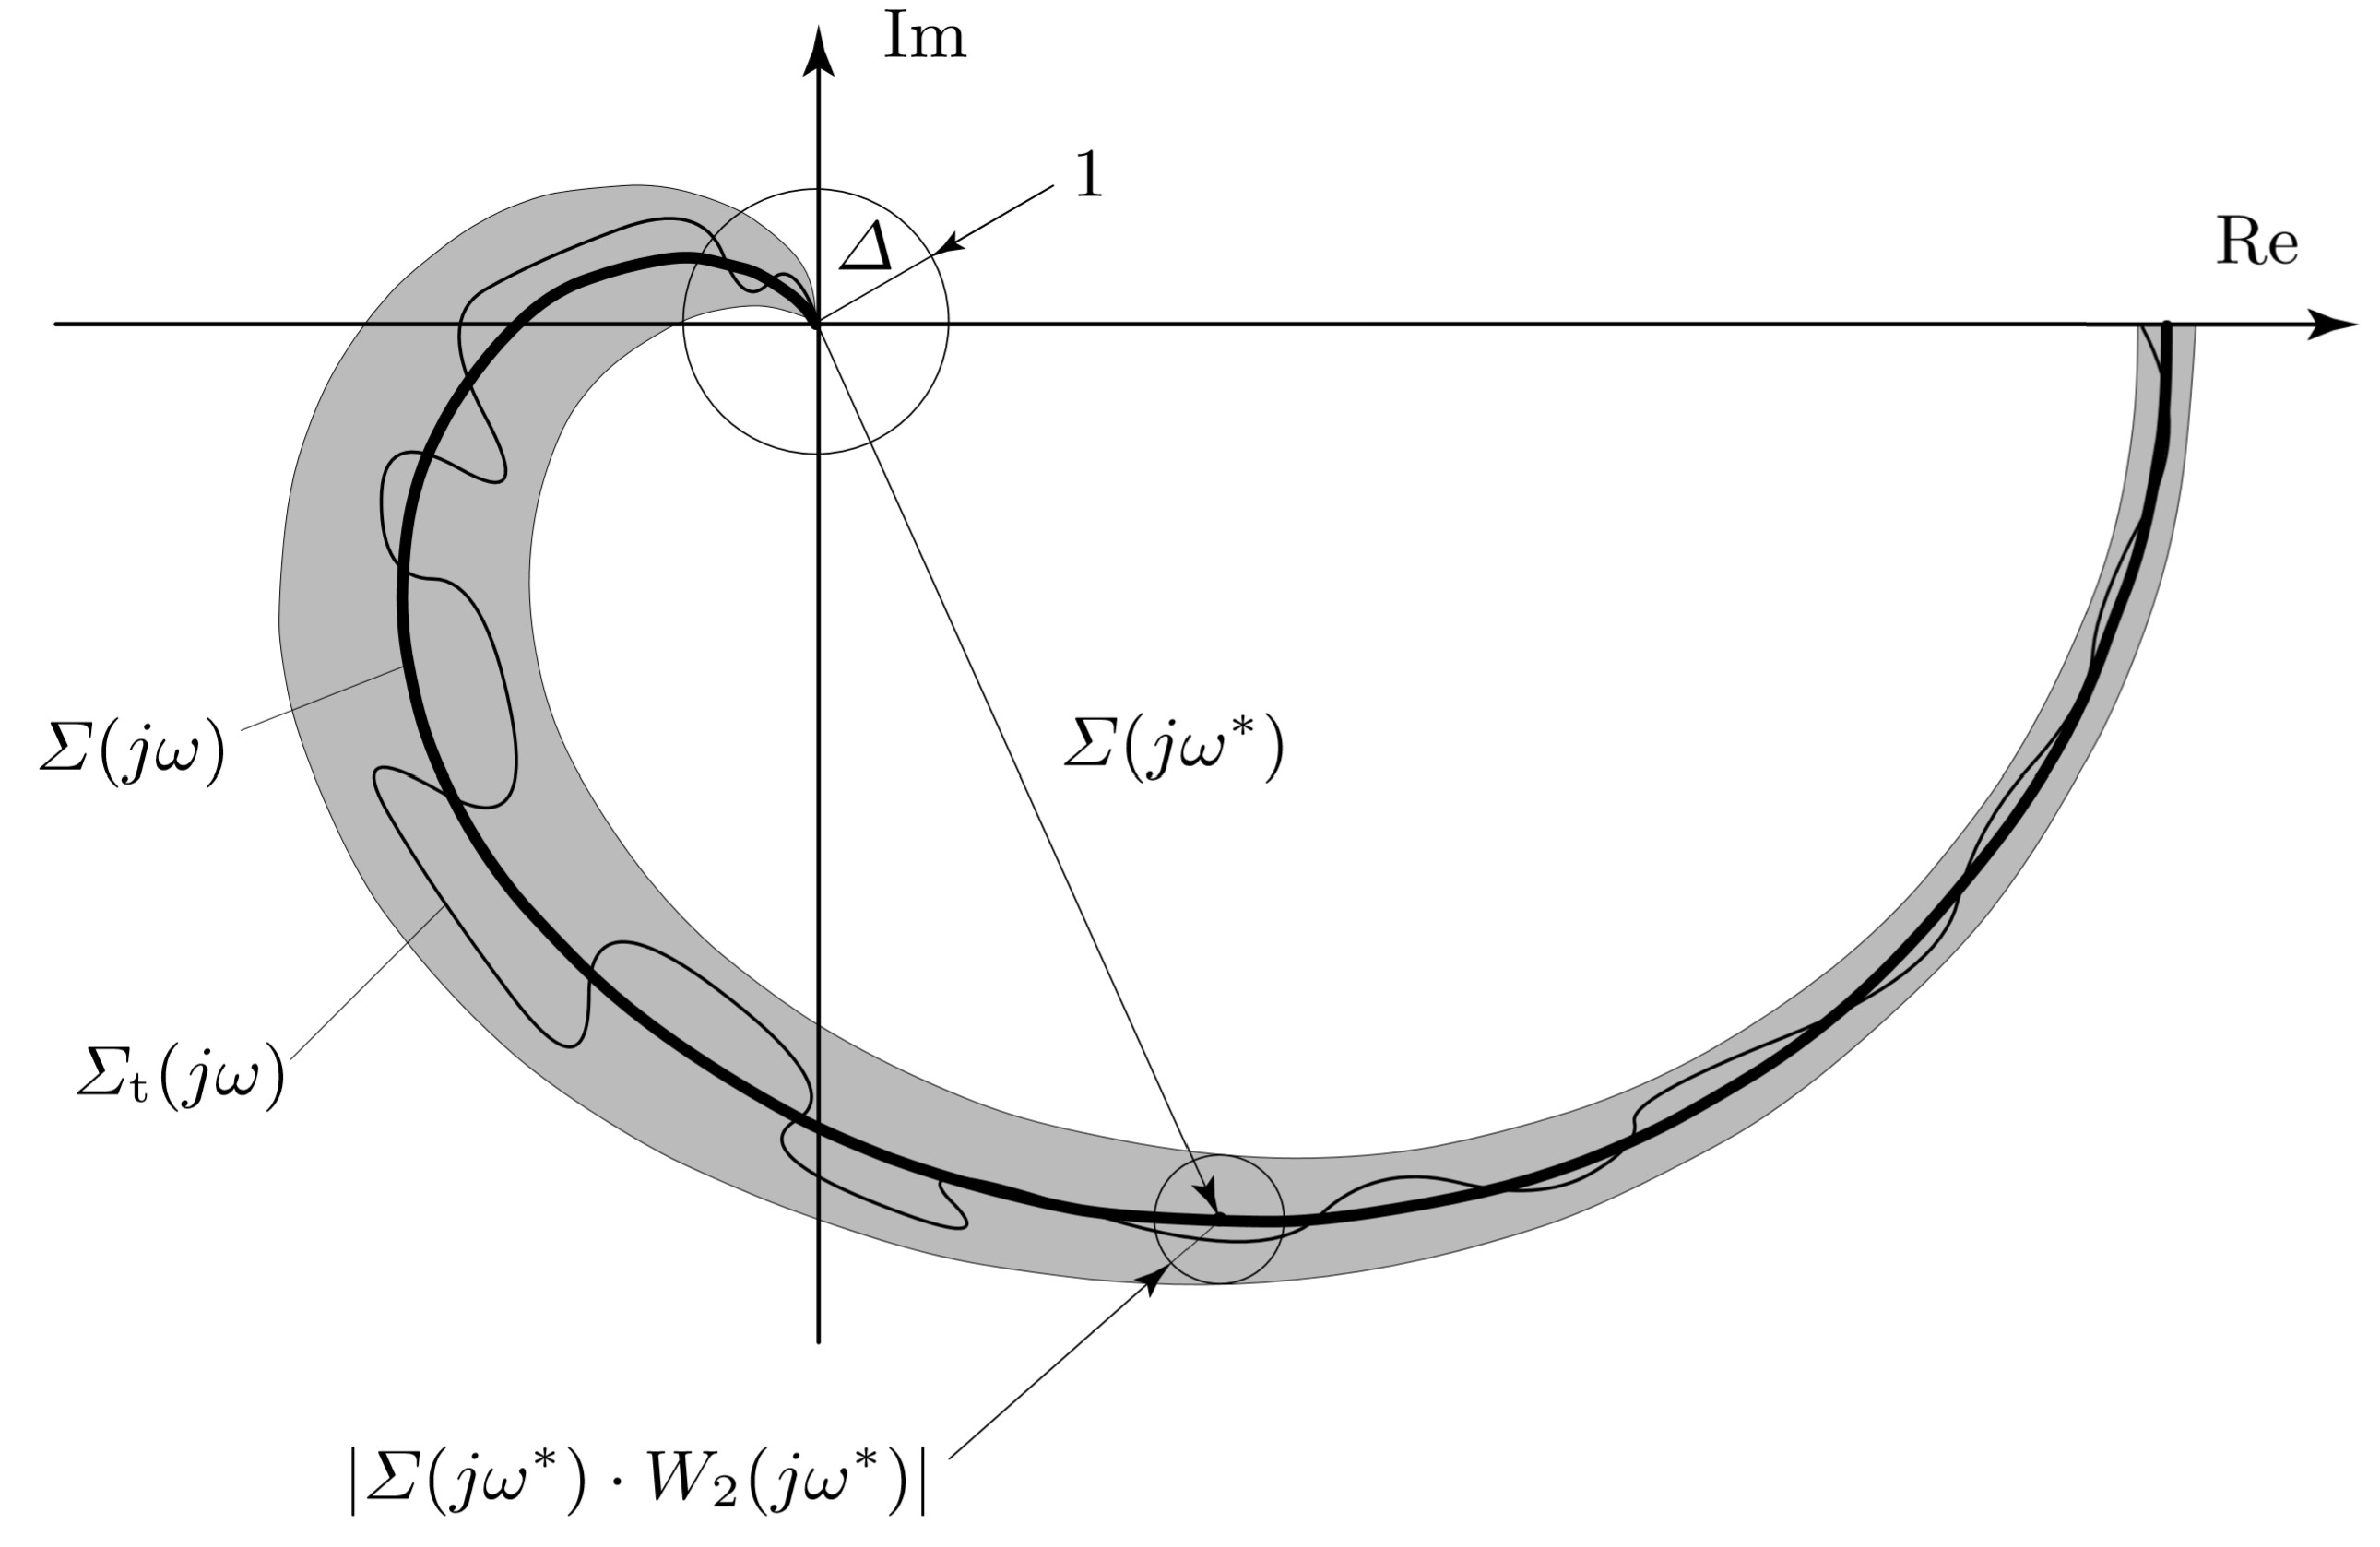
\includegraphics[width = 0.6\linewidth]{images/05/nichtparametrisierte_Unsicherheit.jpg}
            \end{center}
                Annahme: es existiert eine lineare, zeitinvariante wahre Übertragungsfunktion $\Sigma_t(s)$,die das System exakt beschreibt, die jedoch wegen Modellunsicherheiten nicht bekannt ist. Die wahre Übertragungsfunktion $\Sigma(_t(s)$ liegt in der Menge $\mathcal{S}$:
                \[
                \mathcal{S} = \left\{\Sigma(s) \cdot(1+\Delta\cdot W_2(s)) \hspace{3mm} \Delta\begin{cases}  |\Delta| \leq 1\\ \angle \Delta \in[-\pi,\pi]\end{cases}\right\}
                \]
                %alternativ 
                %\mathcal{S} = \{\Sigma(s) \cdot(1+\Delta\cdot W_2(s)) \hspace{3mm} ||\Delta| \leq 1\\ \angle \Delta \in[-\pi,\pi]\}
            
                $\mathbf{\Sigma(S)}$: Nominelle Übertragungsfunktion, durch (imperfekte) Systemodelierung gefunden.
                \\$\mathbf{\Delta}$: Unsicherheitsgenerator: Kreis in der komplexen Ebene.
                \\$\mathbf{W_2(s)}$: Übertragungsfunktion der Unsicherheitsheits: quantifiziert die frequenzabhängige Unsicherheit des Modells
                
                Bei jeder Frequenz $\omega^*$ liegt die wahre Übertragungsfunktion $\Sigma_t(j\omega^*)$innerhalb von einem Kreis mit Radius $|\Sigma(j\omega^*) \cdot W2(j\omega^*|$ um die nominelle Übertragungsfunktion $\Sigma(j\omega^*)$.
            \subsubsection{Unsicherheitsübertragungsfunktion $W_2(s)$}
                Es gibt mehrere Methoden, um ein Modell für die Unsicherheitsübertragungsfunktion zu bestimmen. (Für RT1 ist jedoch nur eine Relevant)
        
               Diese Methode verwendet Messungen am realen System, um die Unsicherheitsgrenzen des Modells davon zu bestimmen:
               
               Vorgehen: 
               \begin{itemize}
                   \item \textbf{Unsicherheitsschätzung mittels Messdaten:}
                   
                   Diese Methode verwendet Messungen am realen System, um die Unsicherheitsgrenzen des Modells davon zu bestimmen.
                \end{itemize}
                   
                   Vorgehen:
                    \begin{enumerate}
                        \item Es werden $k = 1,\hdots,K$ Messungen des Frequenzganges durchgeführt. Für jede Messung bei Frequenz $\omega_i, i =1,\hdots,I$ werden die Werte $|\Sigma(j\omega_{i,k})|$ und $\angle\Sigma(j\omega_{i,k})$ identifiziert.
                        \begin{center}
                            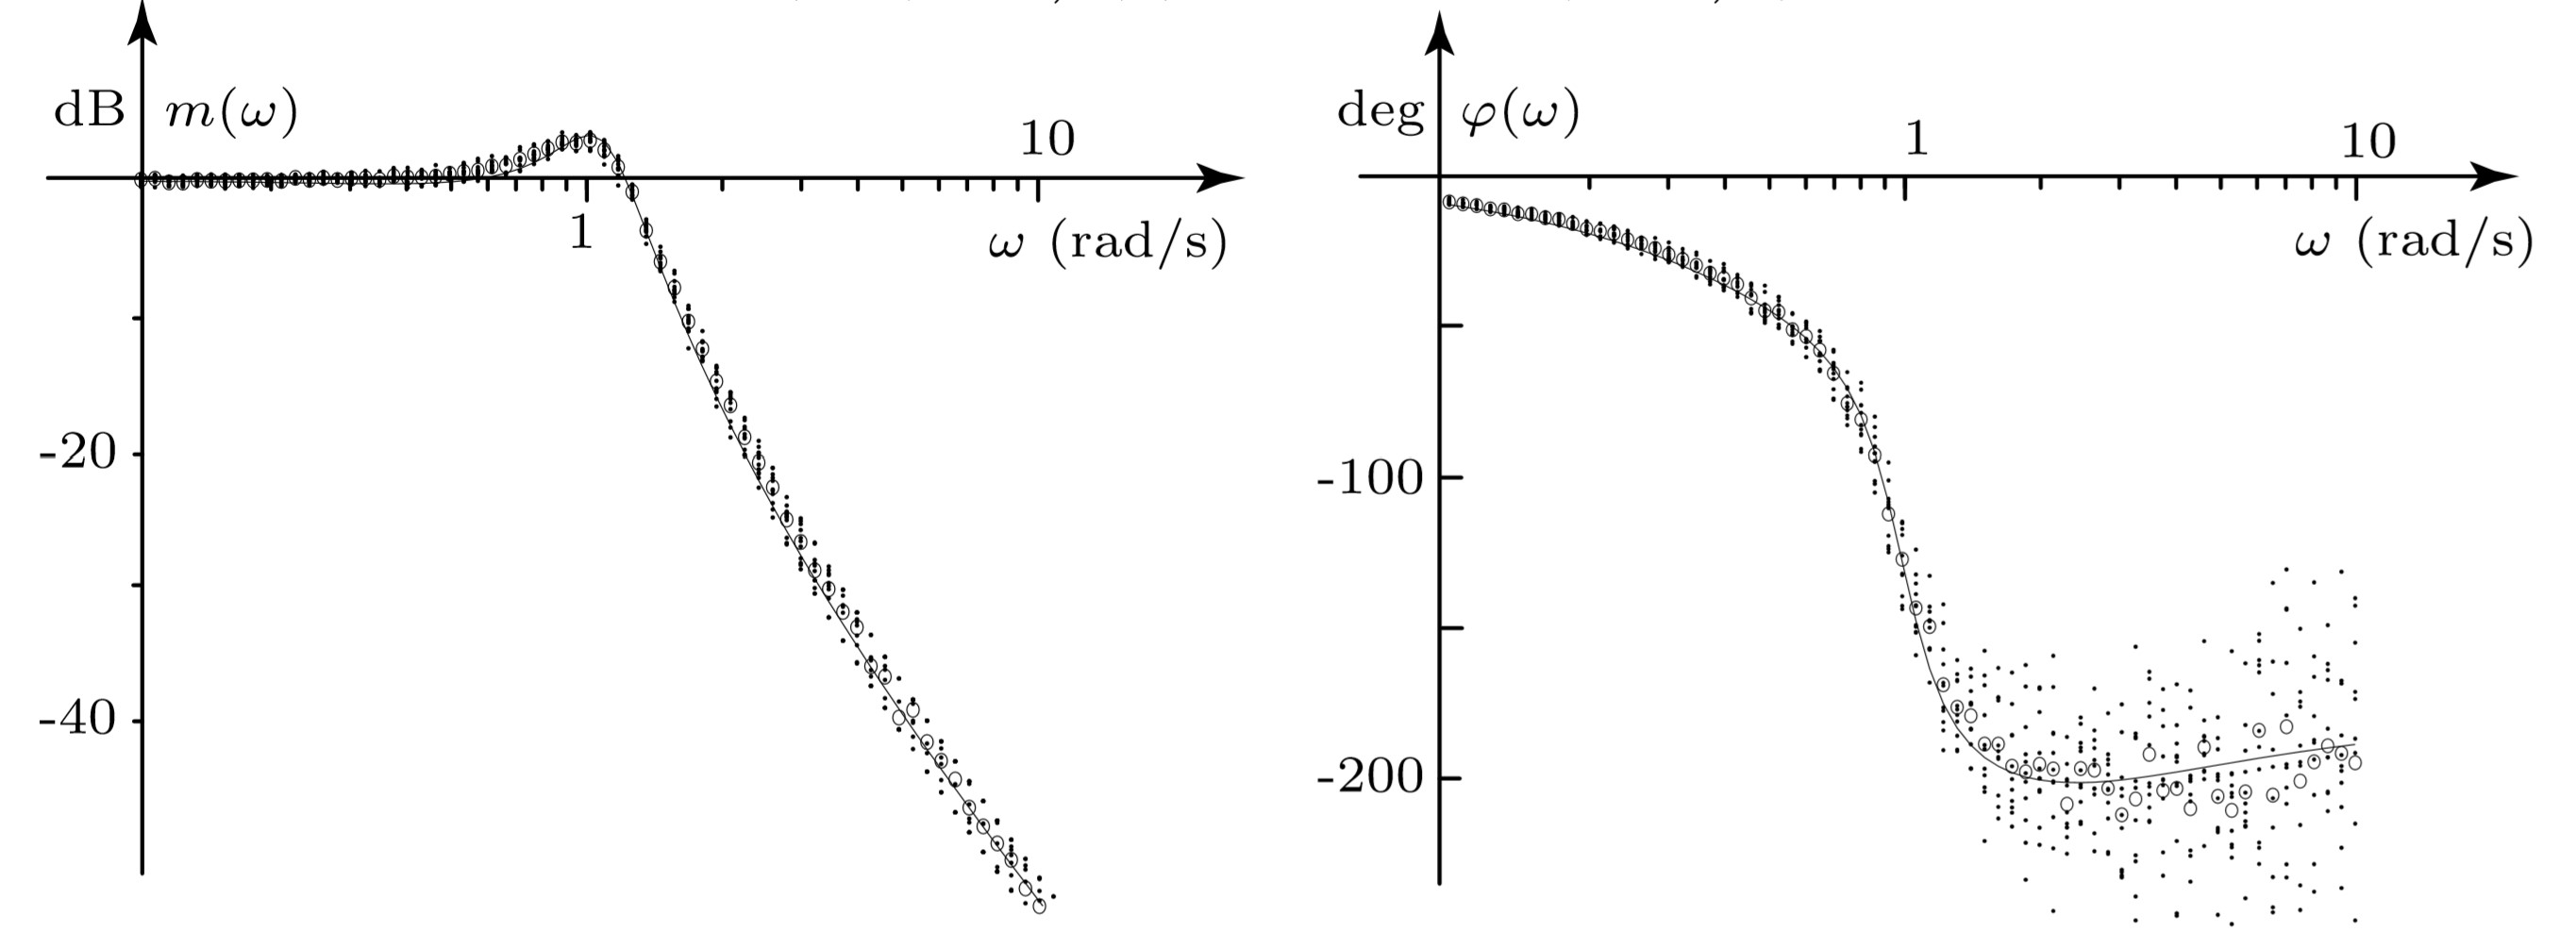
\includegraphics[width = 0.8\linewidth]{images/05/Unsicherheits_Messung.jpg}
                        \end{center}
                        \item Eine nominelle Übertragungsfunktion $\Sigma(s)$ wird an die experimentellen Daten angepasst (analog zur Methode der Systemidentifikation).
                        \[\Sigma(j\omega_i) = m_i \cdot e^{j\cdot\varphi_i}\]
                        \item  Bei jeder Frequenz $\omega_i$ sind die Werte der $K$ Messungen von $|\Sigma(j\omega_{i,k})|$ verteilt um den Wert der nominellen Übertragungsfunktion $|\Sigma(j\omega_i)|$. Die Unsicherheitsübertragungsfunktion bildet einen Kreis mit Radius $|W_2(j\omega_i)|$ um $|\Sigma(j\omega_i)|$ so dass alle Messpunkte von $|\Sigma(j\omega_{i,k})|$ darin enthalten sind:
                        \[\frac{\Sigma(j\omega_{i,k})}{\Sigma(j\omega_i)}-1 < |W_2(j\omega_i)|k\in [1,K] i \in[1,I]\]
                        
                        Die Ungleichung definiert eine Bedingung bei jeder Frequenz $\omega_i$. Wird die Linke Seite der Ungleichung als Funktion der Frequenz dargestellt, ergibt sich:
                        \begin{center}
                            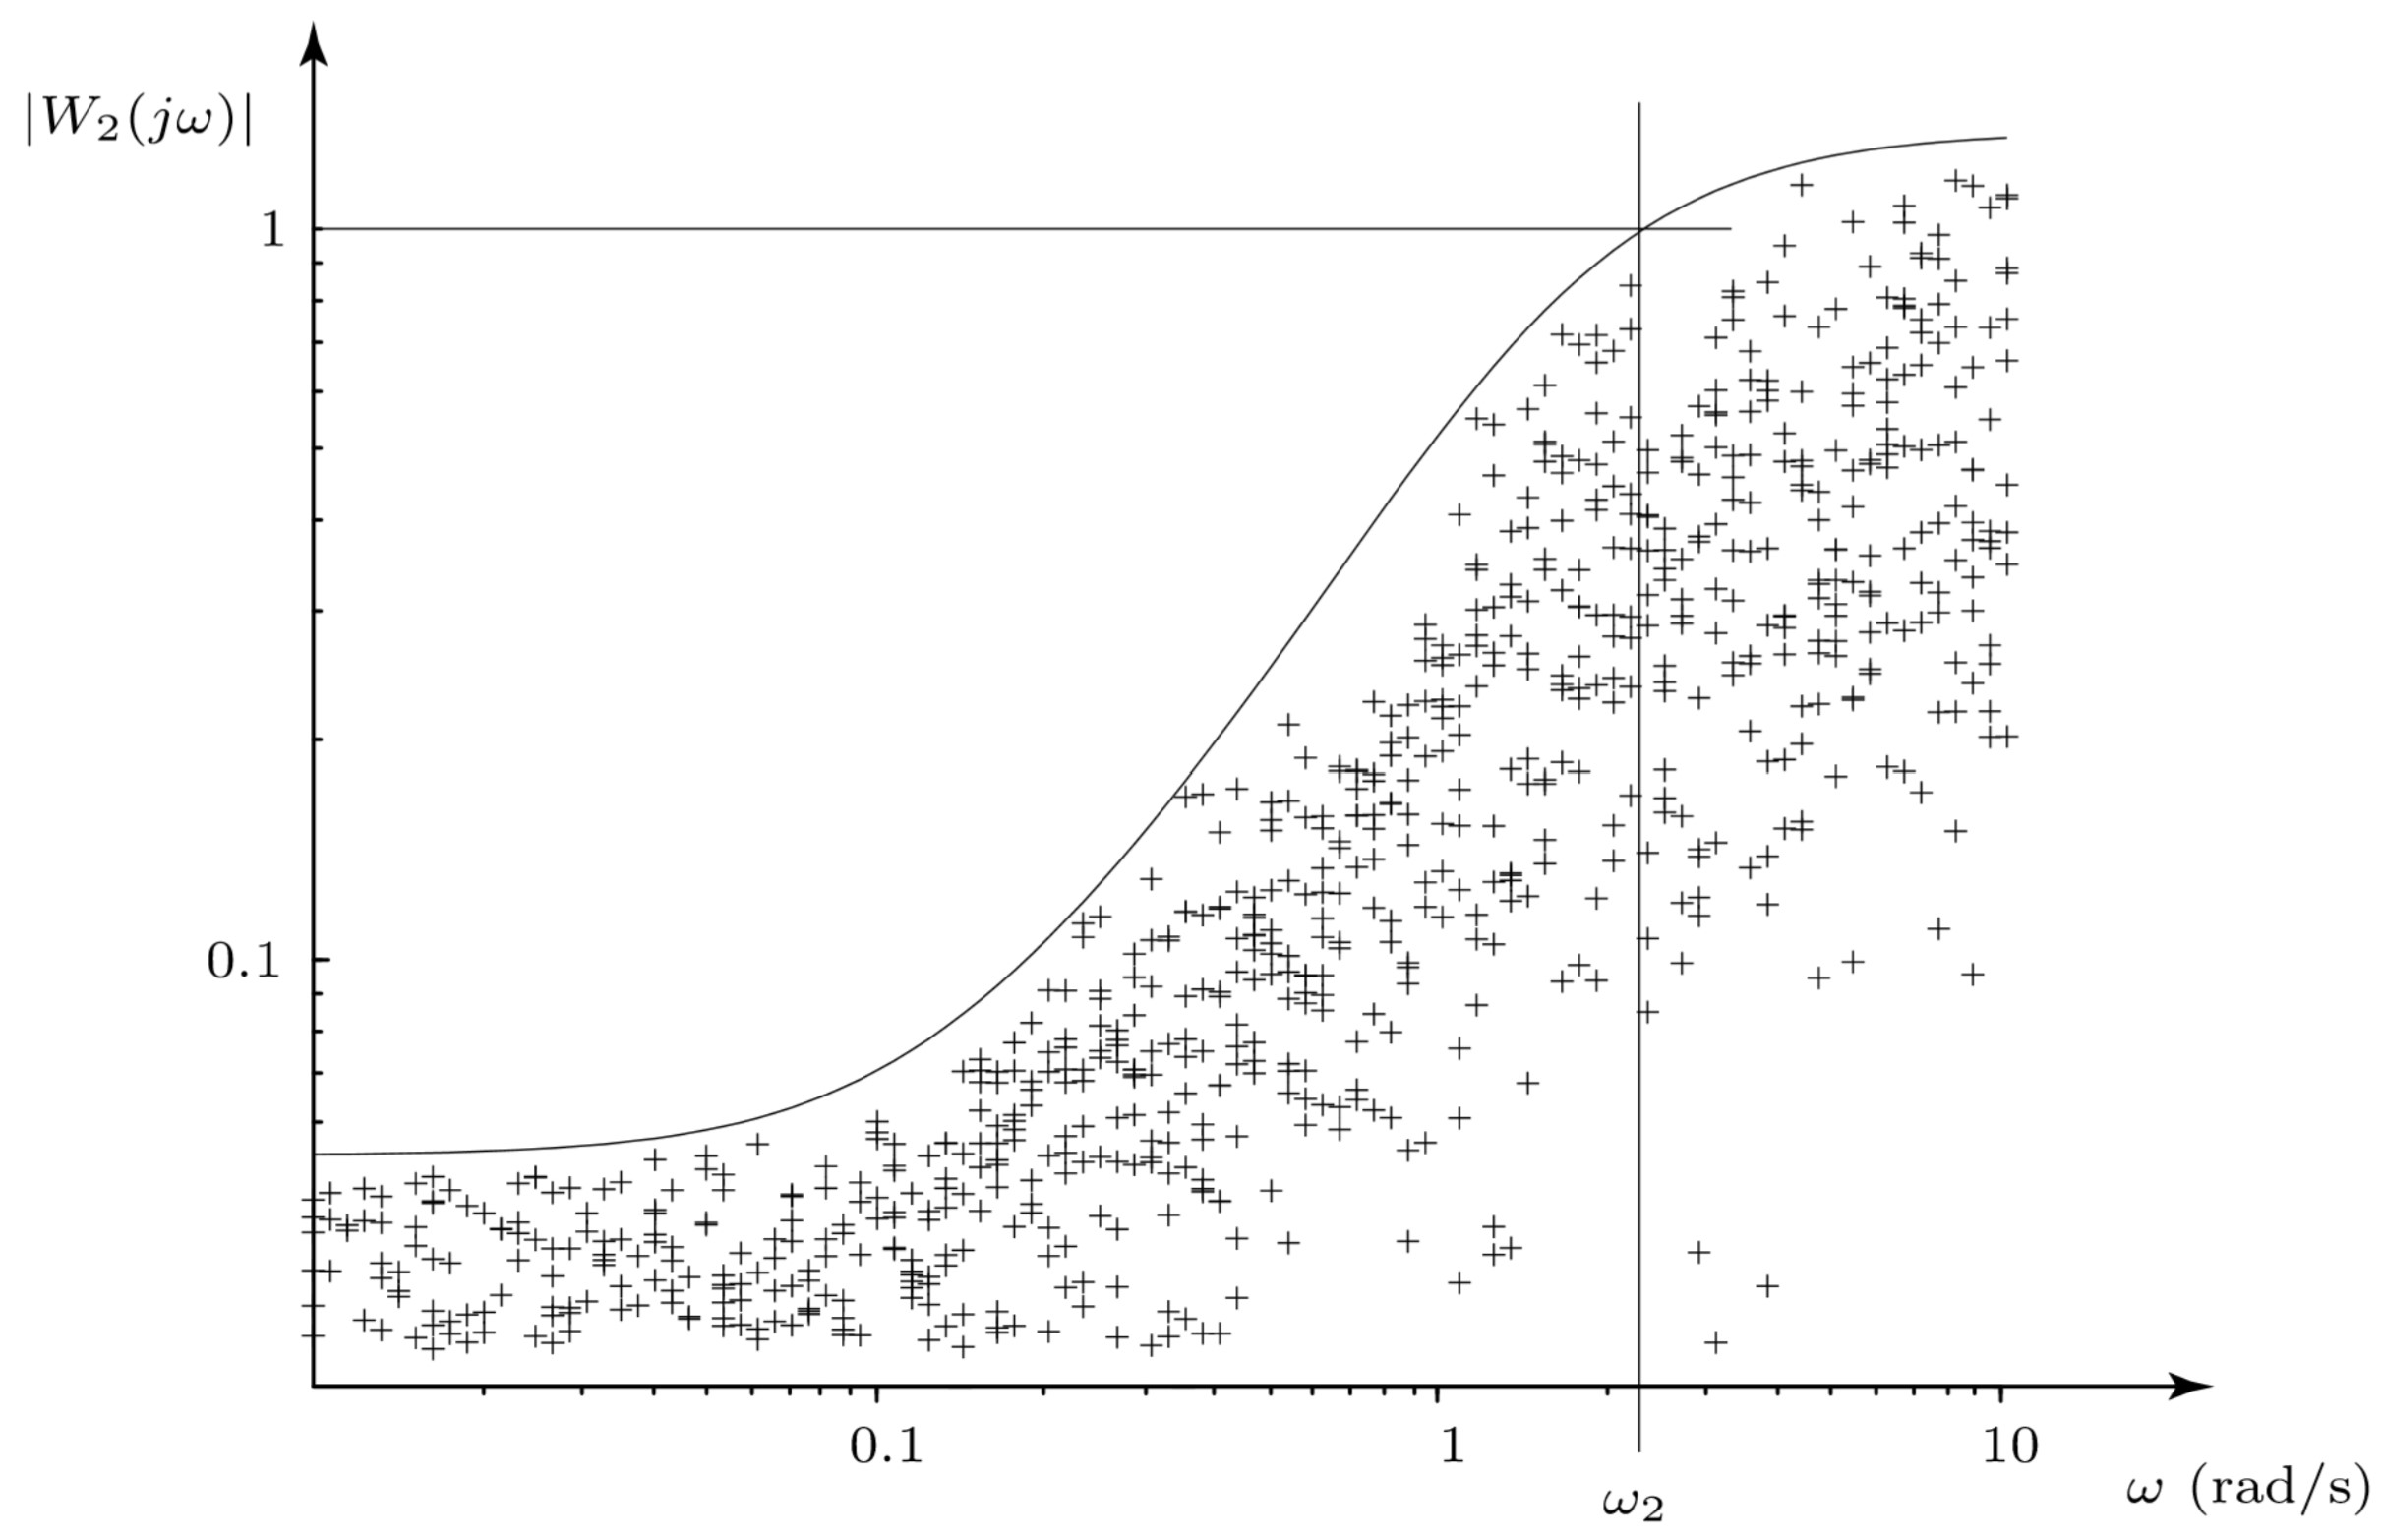
\includegraphics[width = 0.65\linewidth]{images/05/UnsicherheitsFunktion.jpg}
                        \end{center}
                        \textbf{Bemerkungen:} 
                        
                        Die Unsicherheit steigt bei höheren Frequenzen, den Daten kann eine Unsicherheitsübertragungsfunktion $W_2(s)$ zugeordnet werden.
                        
                        Die Unsicherheitsübertragungsfunktion $W_2(s)$ enthält keine Phaseninformation.
                        

                    \end{enumerate}
                    %nicht relevant für RT1
                    % \item\textbf{approximation durch varieren der Parameter}
                    
                    % Eine Mathemathische Greybox-model wurde ermittelt und alle Parameter sind bekannt und liegen in bestimmten Intervallen.
                    
                    % \begin{enumerate}
                    %     \item Mit diesen Daten kann ein groben Ansatz gemacht werden, bei dem die Parameter-Intervalle im finiten Gitter abgedeckt ("covered" - geplotted?) werden und dann in einem zweiten Schritt die Frequenzantwort von allen Gitter Punkten berechnet wird.
                    %     \item Weiter vorgehen wie bei \textit{Unsicherheitsschätzung mittels Messdaten}
                    % \end{enumerate}
                    % \item\textbf{Unsicherheit durch simplifiziertes Modell:}
                    % Ein mathematisches Modell von einer Strecke ist bekannt, jedoch zu komplex für das designen eines Kontrollsystems. Ziel ist es das Modell mit einem simpleren Modell in Kombination mit einer Unsicherheitsschranke zu approximieren, welche das ursprüngliche komplexe Modell beinhaltet